\begin{itemize}
    \item \textbf{Diagramas de Flujo (Cliente.c)}
\end{itemize}

\setcounter{figure}{0} % La siguiente figura será la número 1

\begin{figure}[H]
    \centering
    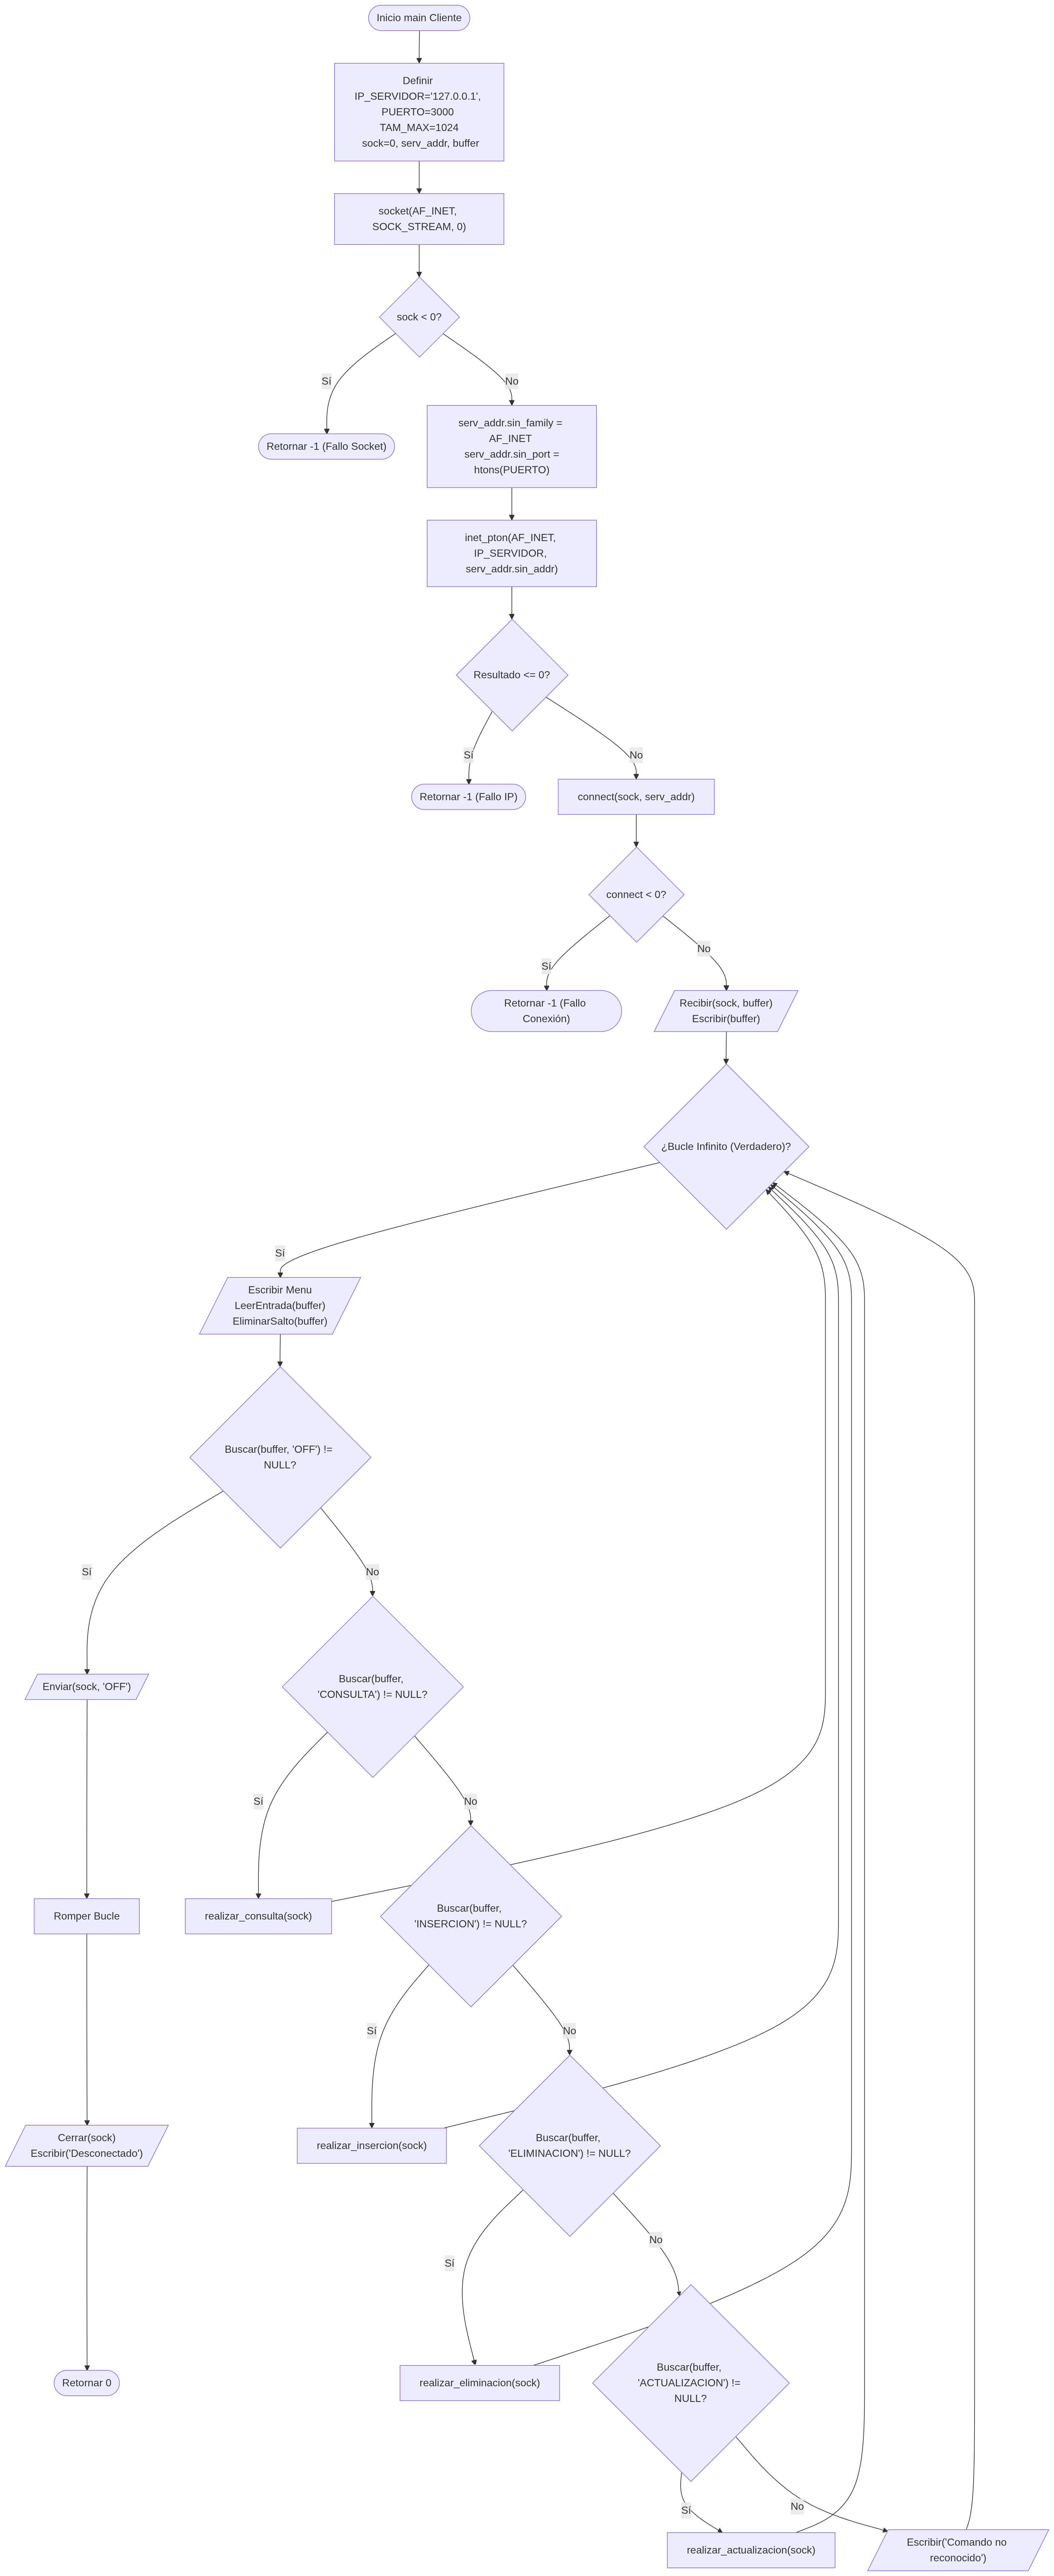
\includegraphics[width=0.49\textwidth]{Cliente/main.png} 
    \caption{Cliente/main}
\end{figure}

\begin{figure}[H]
    \centering
    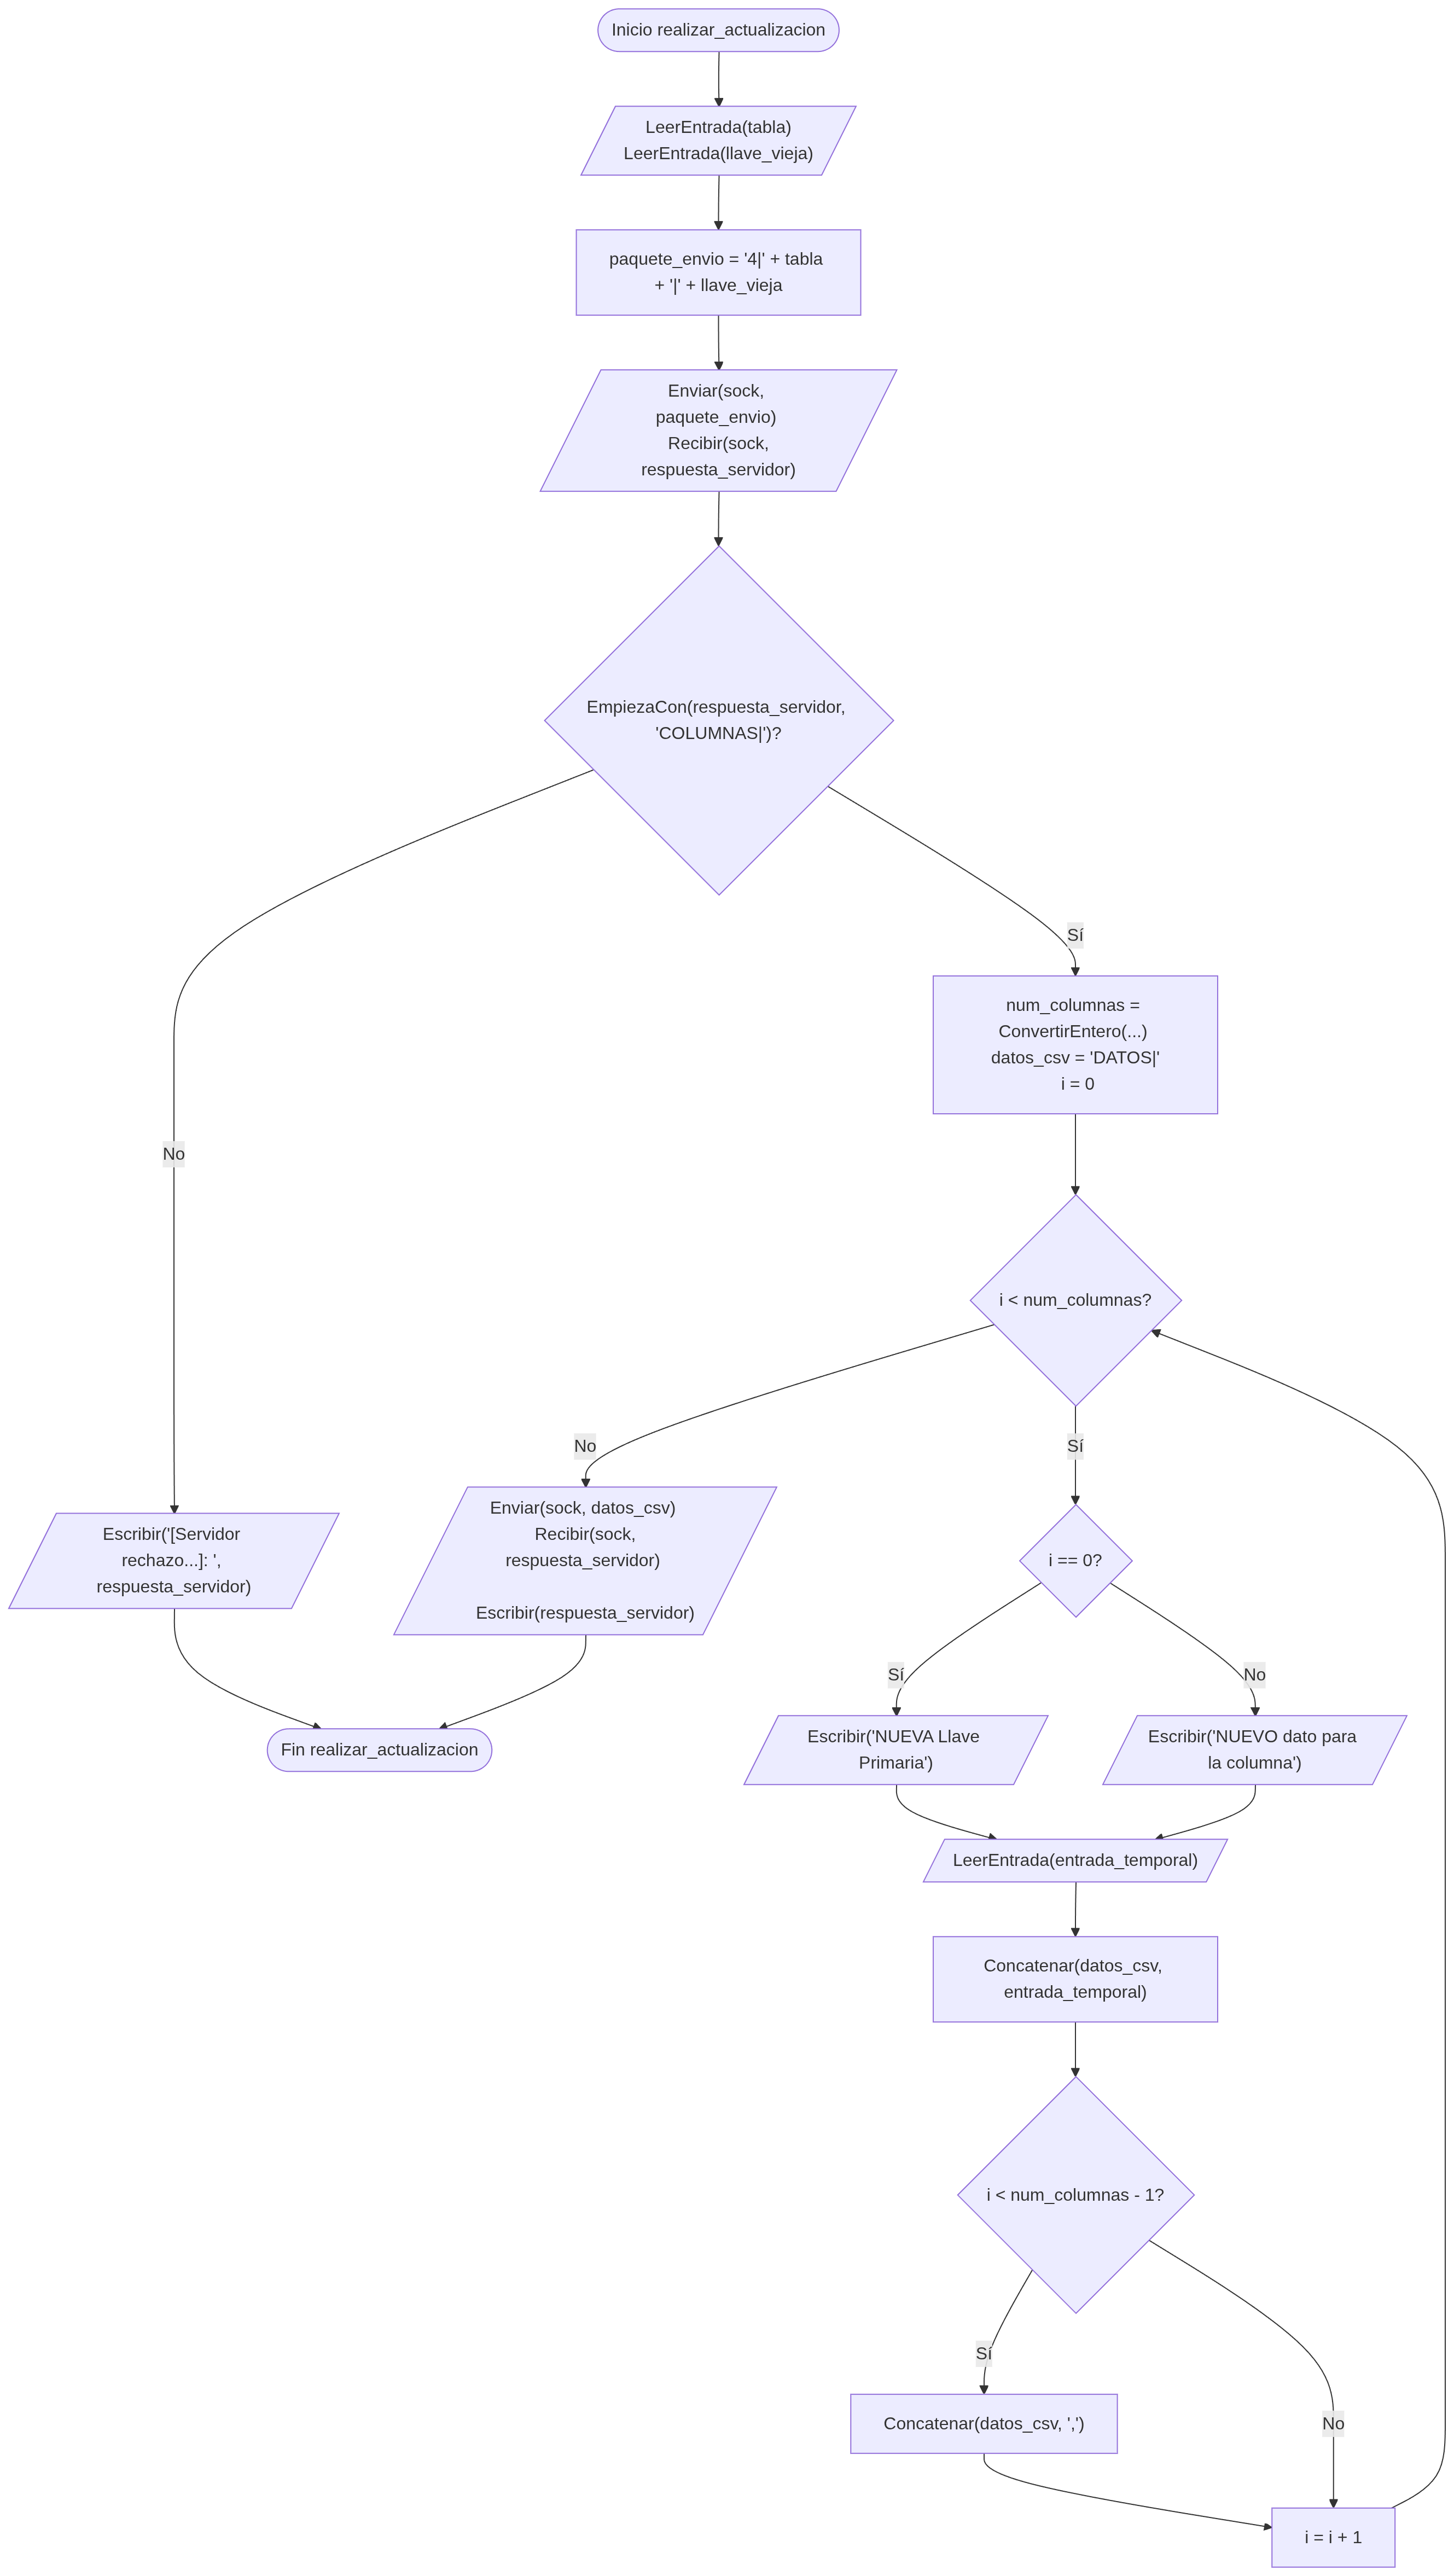
\includegraphics[width=0.65\textwidth]{Cliente/realizar_actualizacion.png} 
    \caption{Cliente/realizar\_actualizacion}
\end{figure}

\begin{figure}[H]
    \centering
    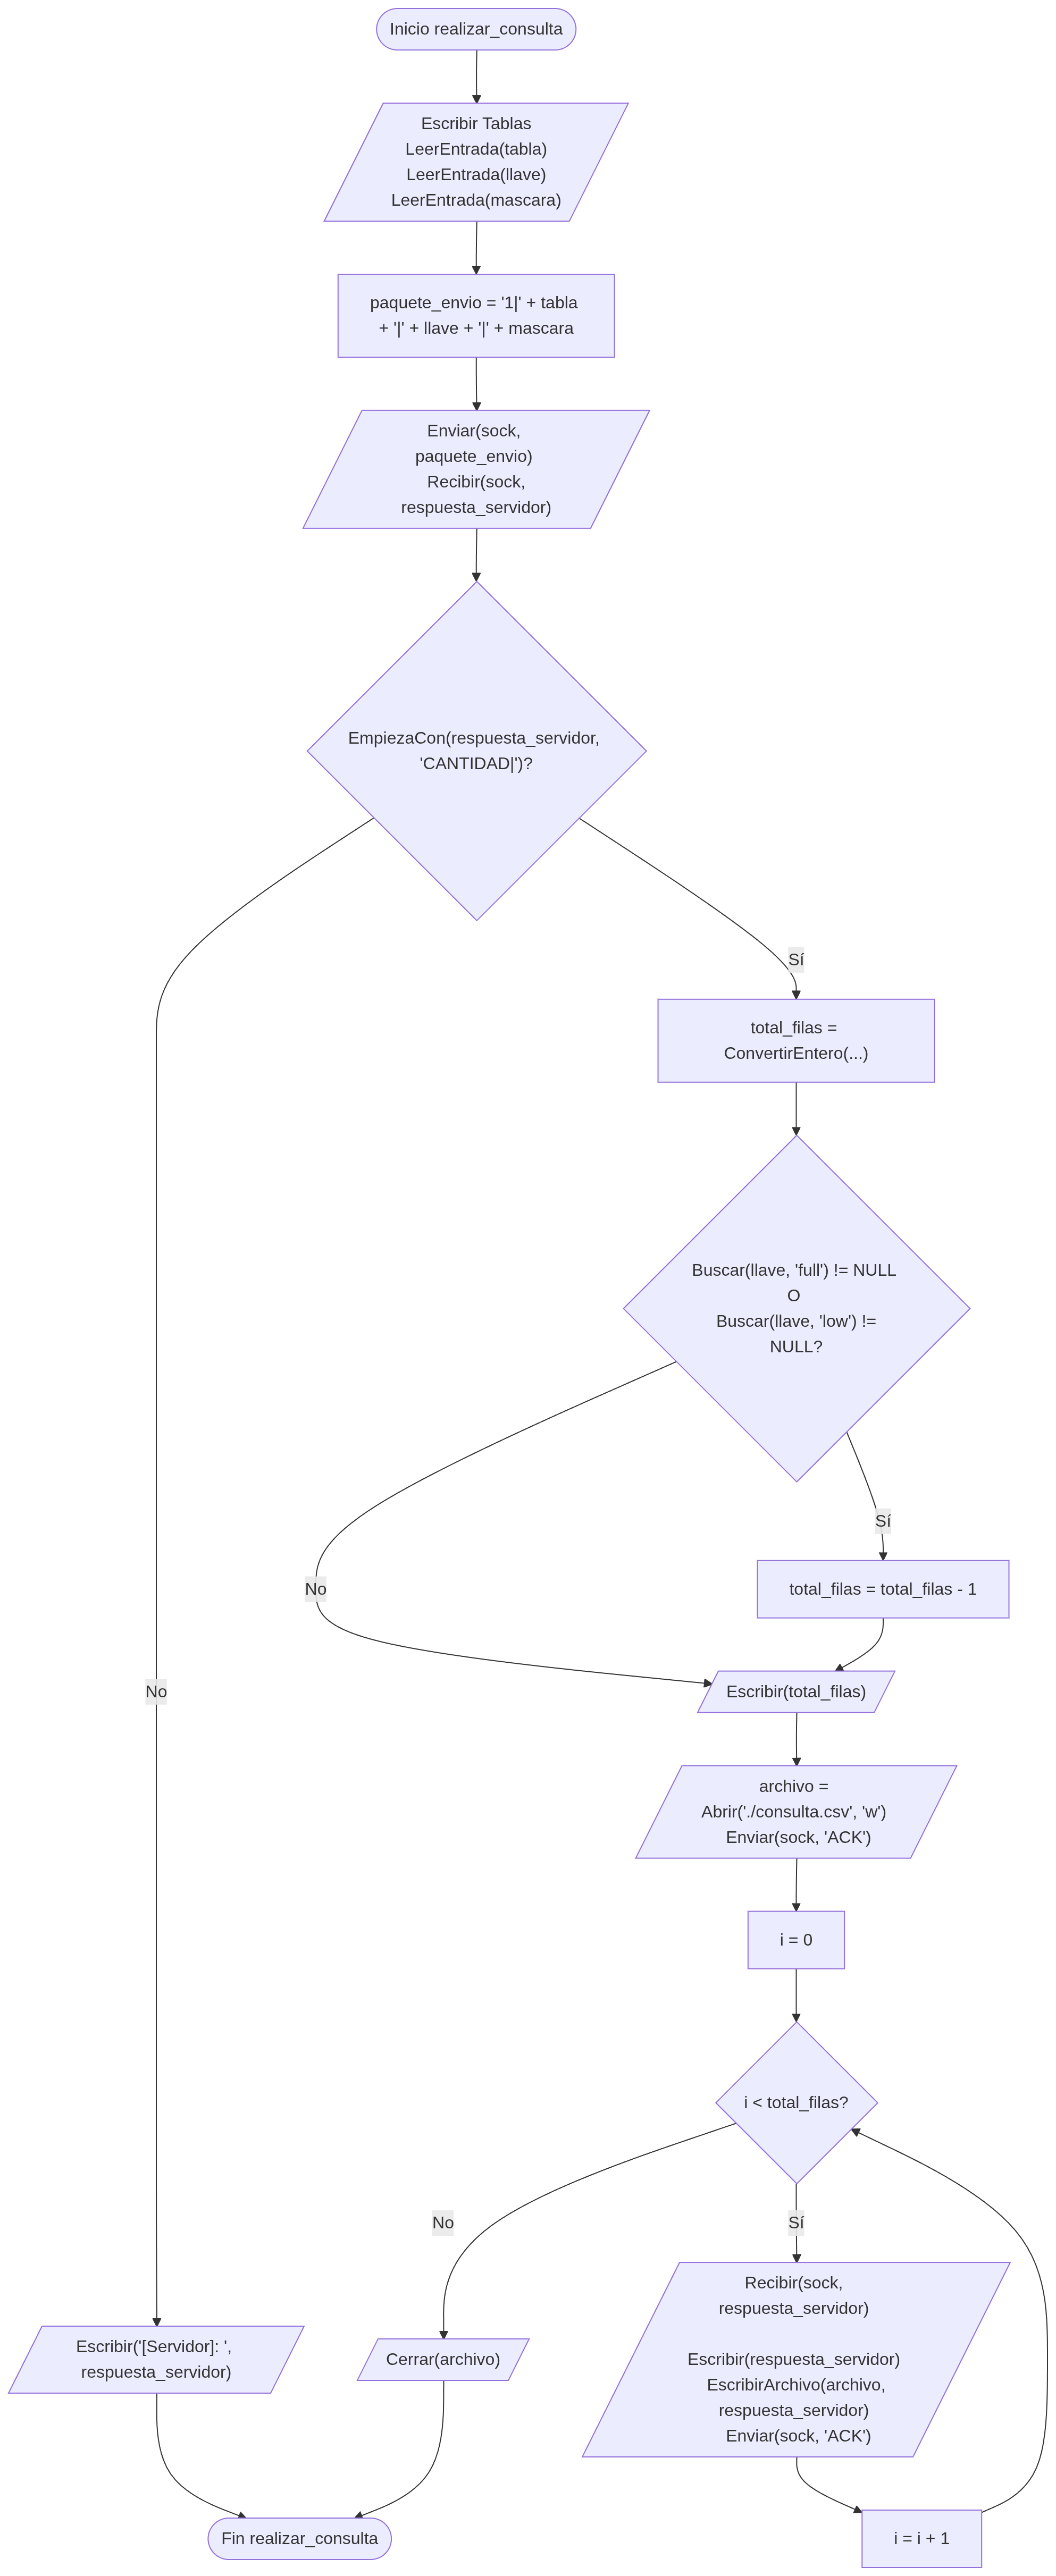
\includegraphics[width=0.48\textwidth]{Cliente/realizar_consulta.png} 
    \caption{Cliente/realizar\_consulta}
\end{figure}

\begin{figure}[H]
    \centering
    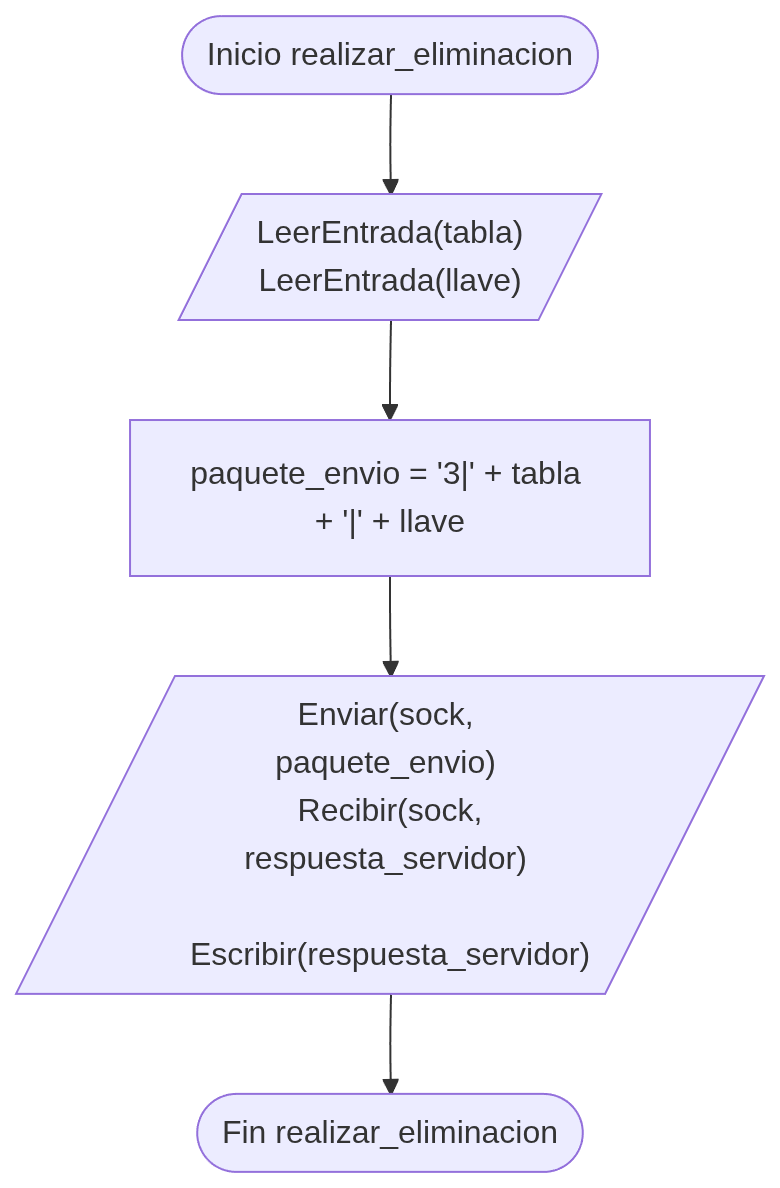
\includegraphics[width=0.48\textwidth]{Cliente/realizar_eliminacion.png} 
    \caption{Cliente/realizar\_eliminacion}
\end{figure}s

\begin{figure}[H]
    \centering
    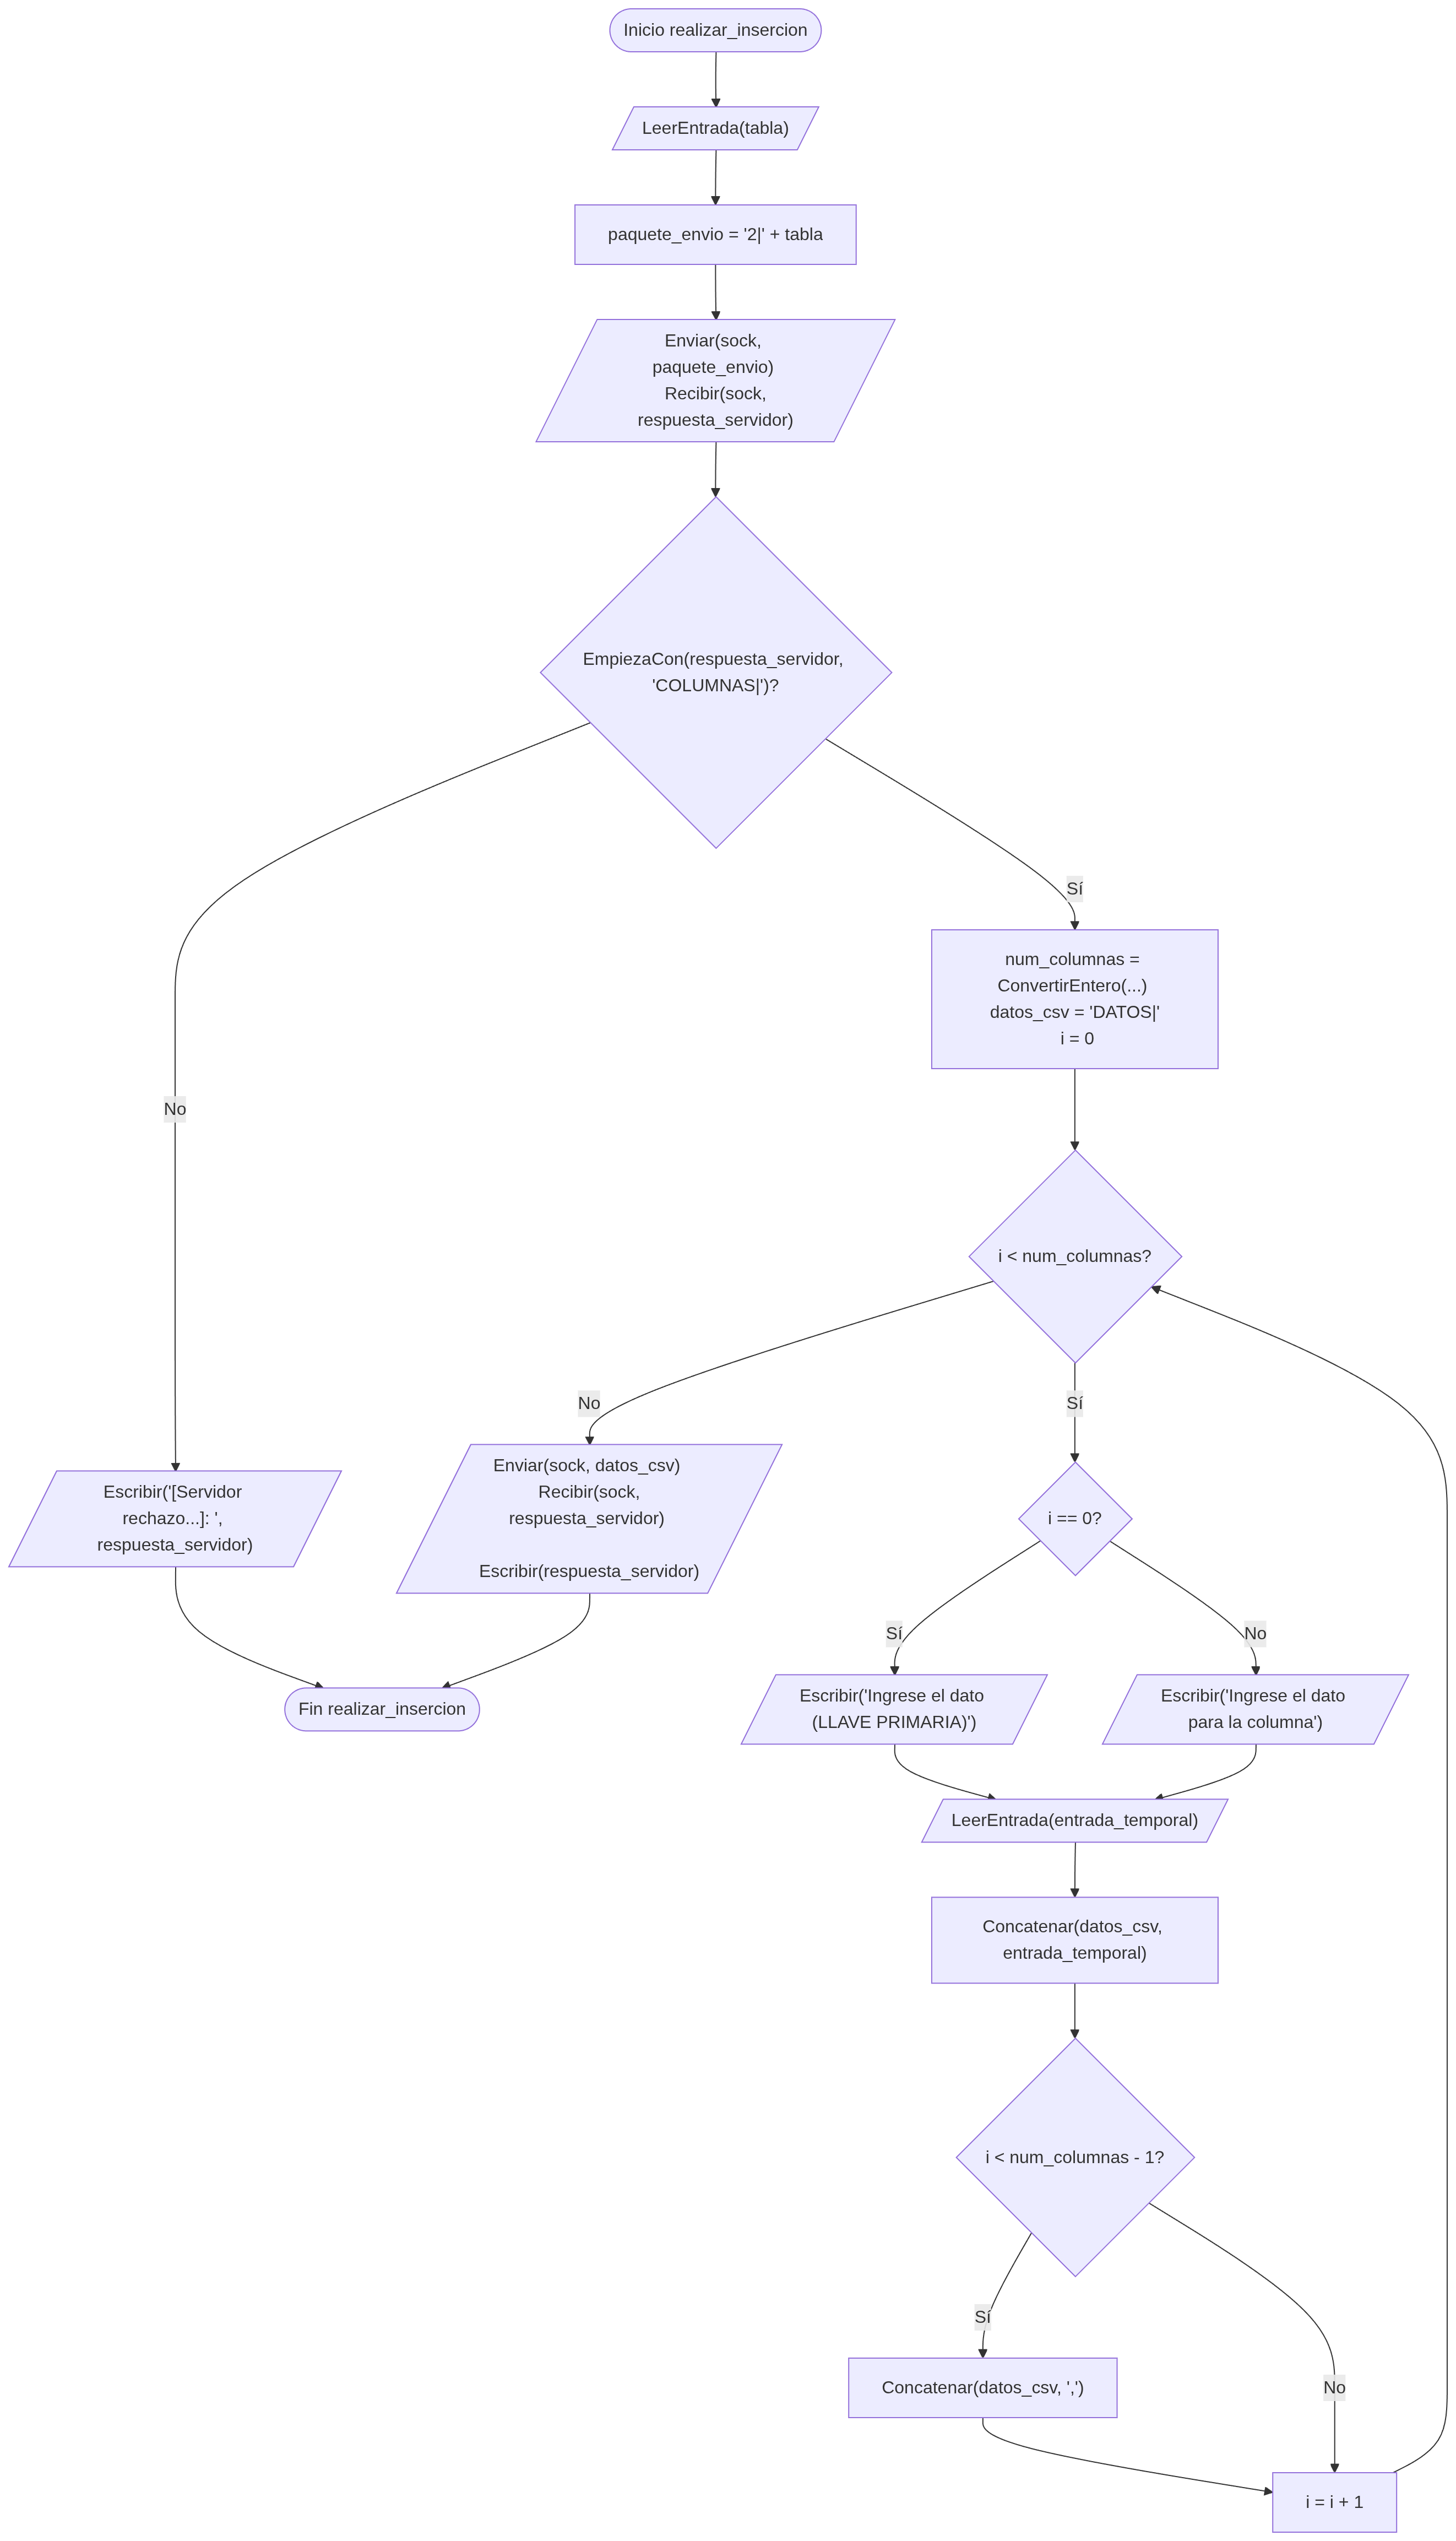
\includegraphics[width=0.65\textwidth]{Cliente/realizar_insercion.png} 
    \caption{Cliente/realizar\_insercion}
\end{figure}

\begin{itemize}
    \item \textbf{Diagrama de Flujo (Servidor.c)}
\end{itemize}

\setcounter{figure}{0} % La siguiente figura será la número 1

\begin{figure}[H]
    \centering
    \includegraphics[width=0.65\textwidth]{Servidor/servidor.png} 
    \caption{Servidor.c}
\end{figure}

\begin{itemize}
    \item \textbf{Diagrama de Flujo (funciones.c)}
\end{itemize}

\setcounter{figure}{0} % La siguiente figura será la número 1

\begin{figure}[H]
    \centering
    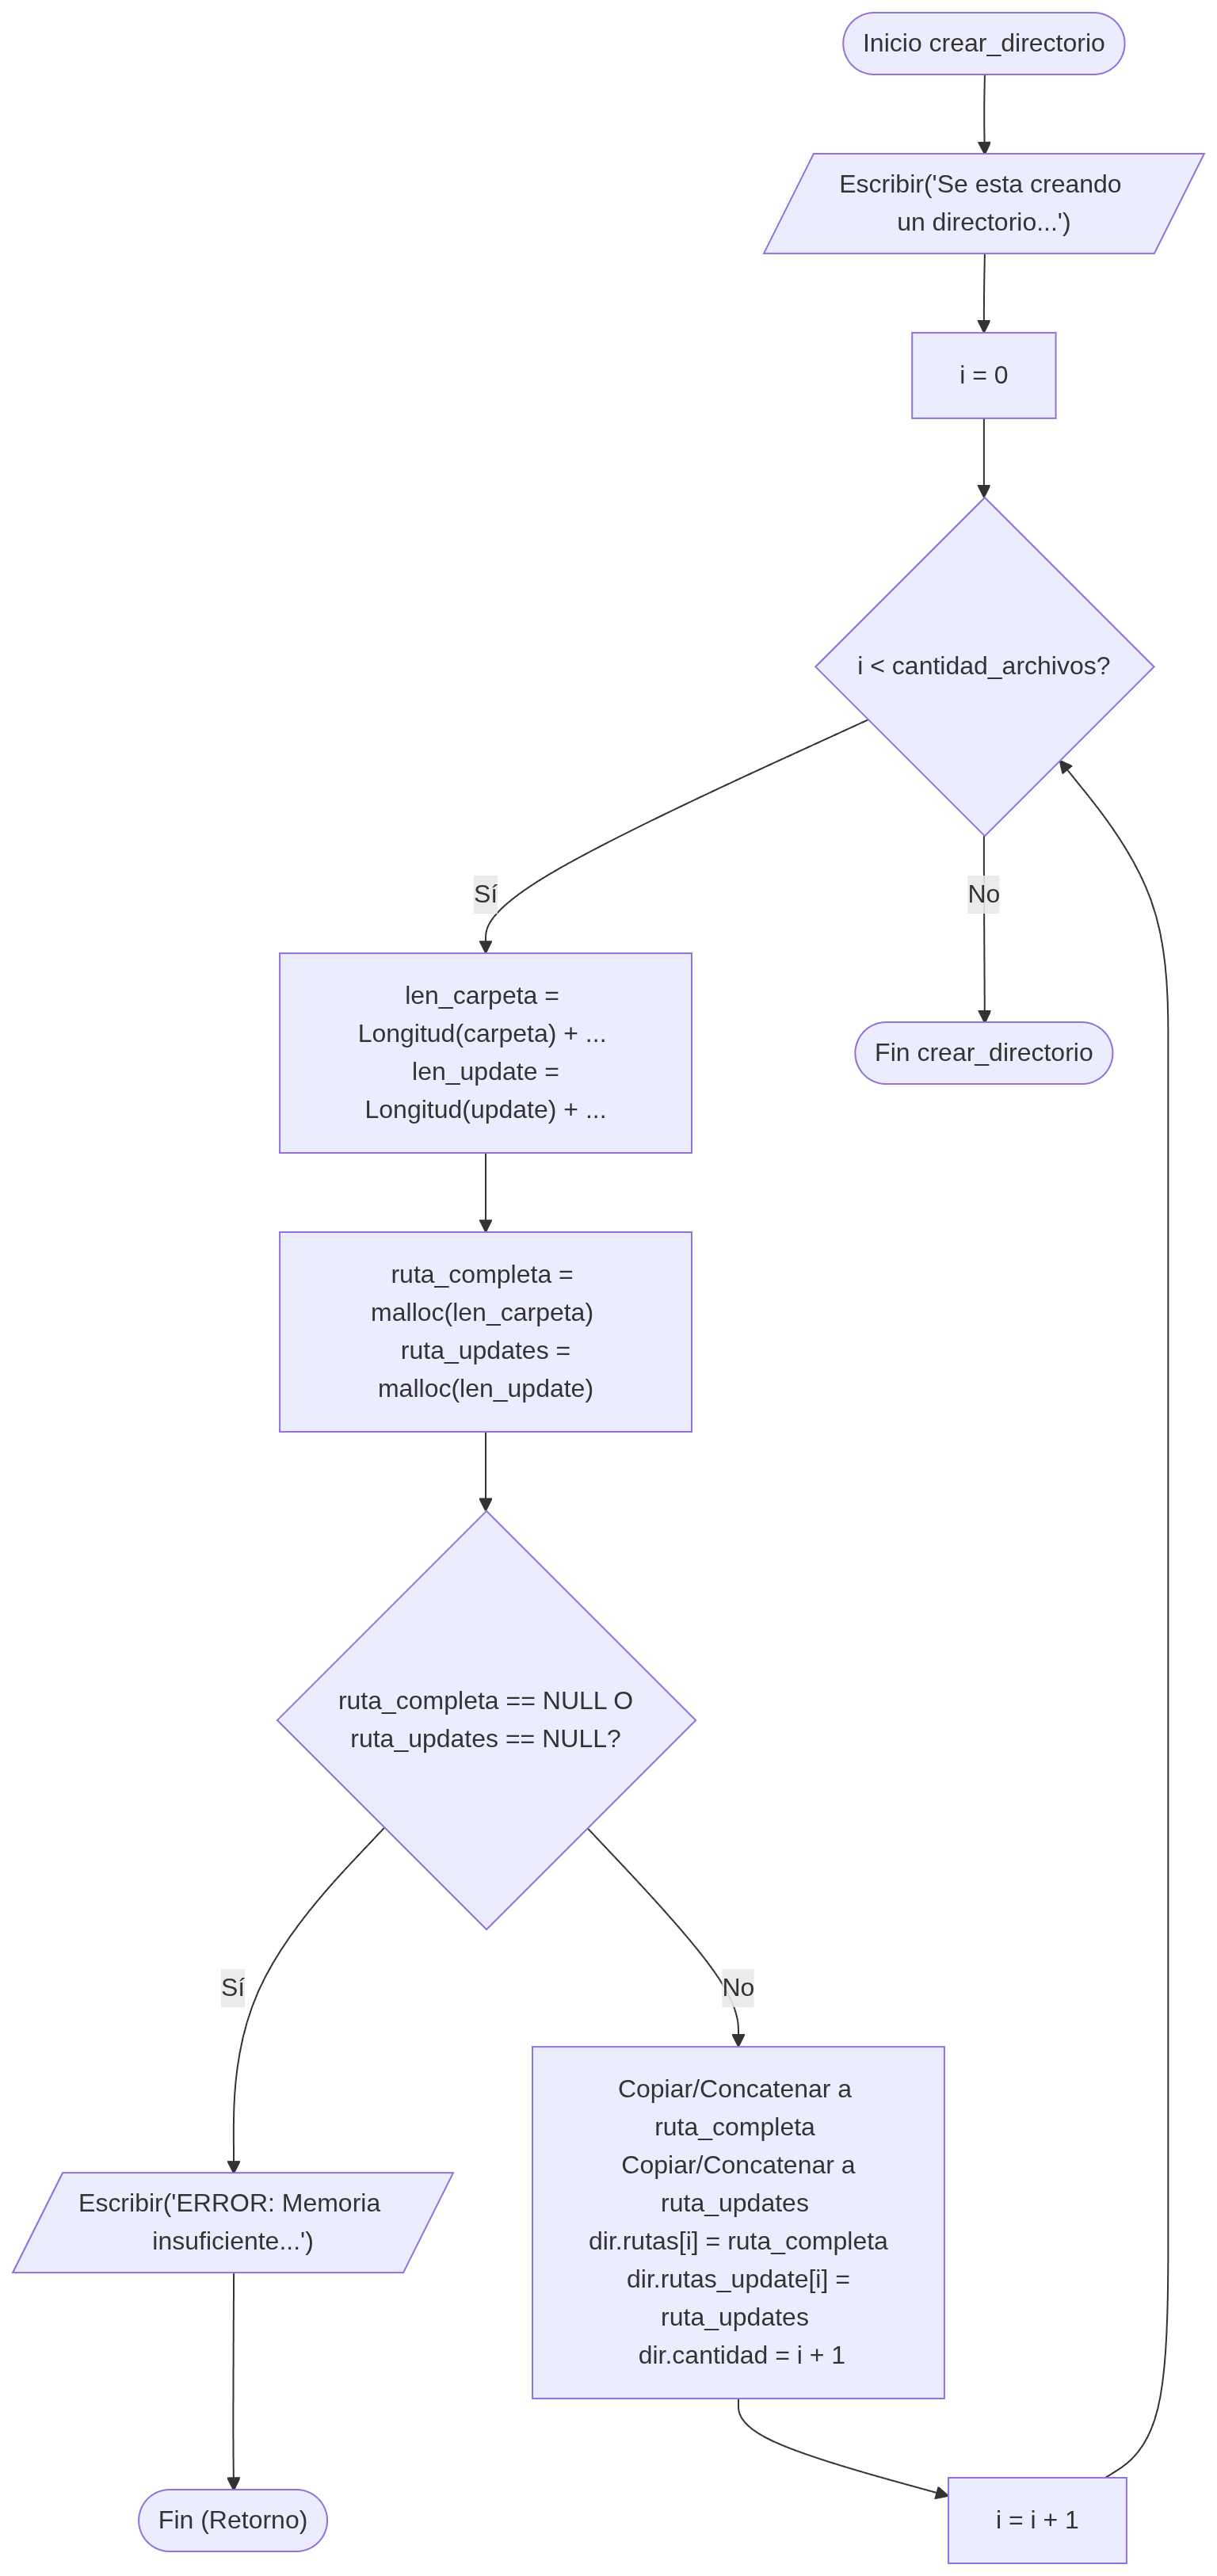
\includegraphics[width=0.45\textwidth]{funciones/crear_directorio.png} 
    \caption{funciones.c/crear\_directorio}
\end{figure}

\begin{figure}[H]
    \centering
    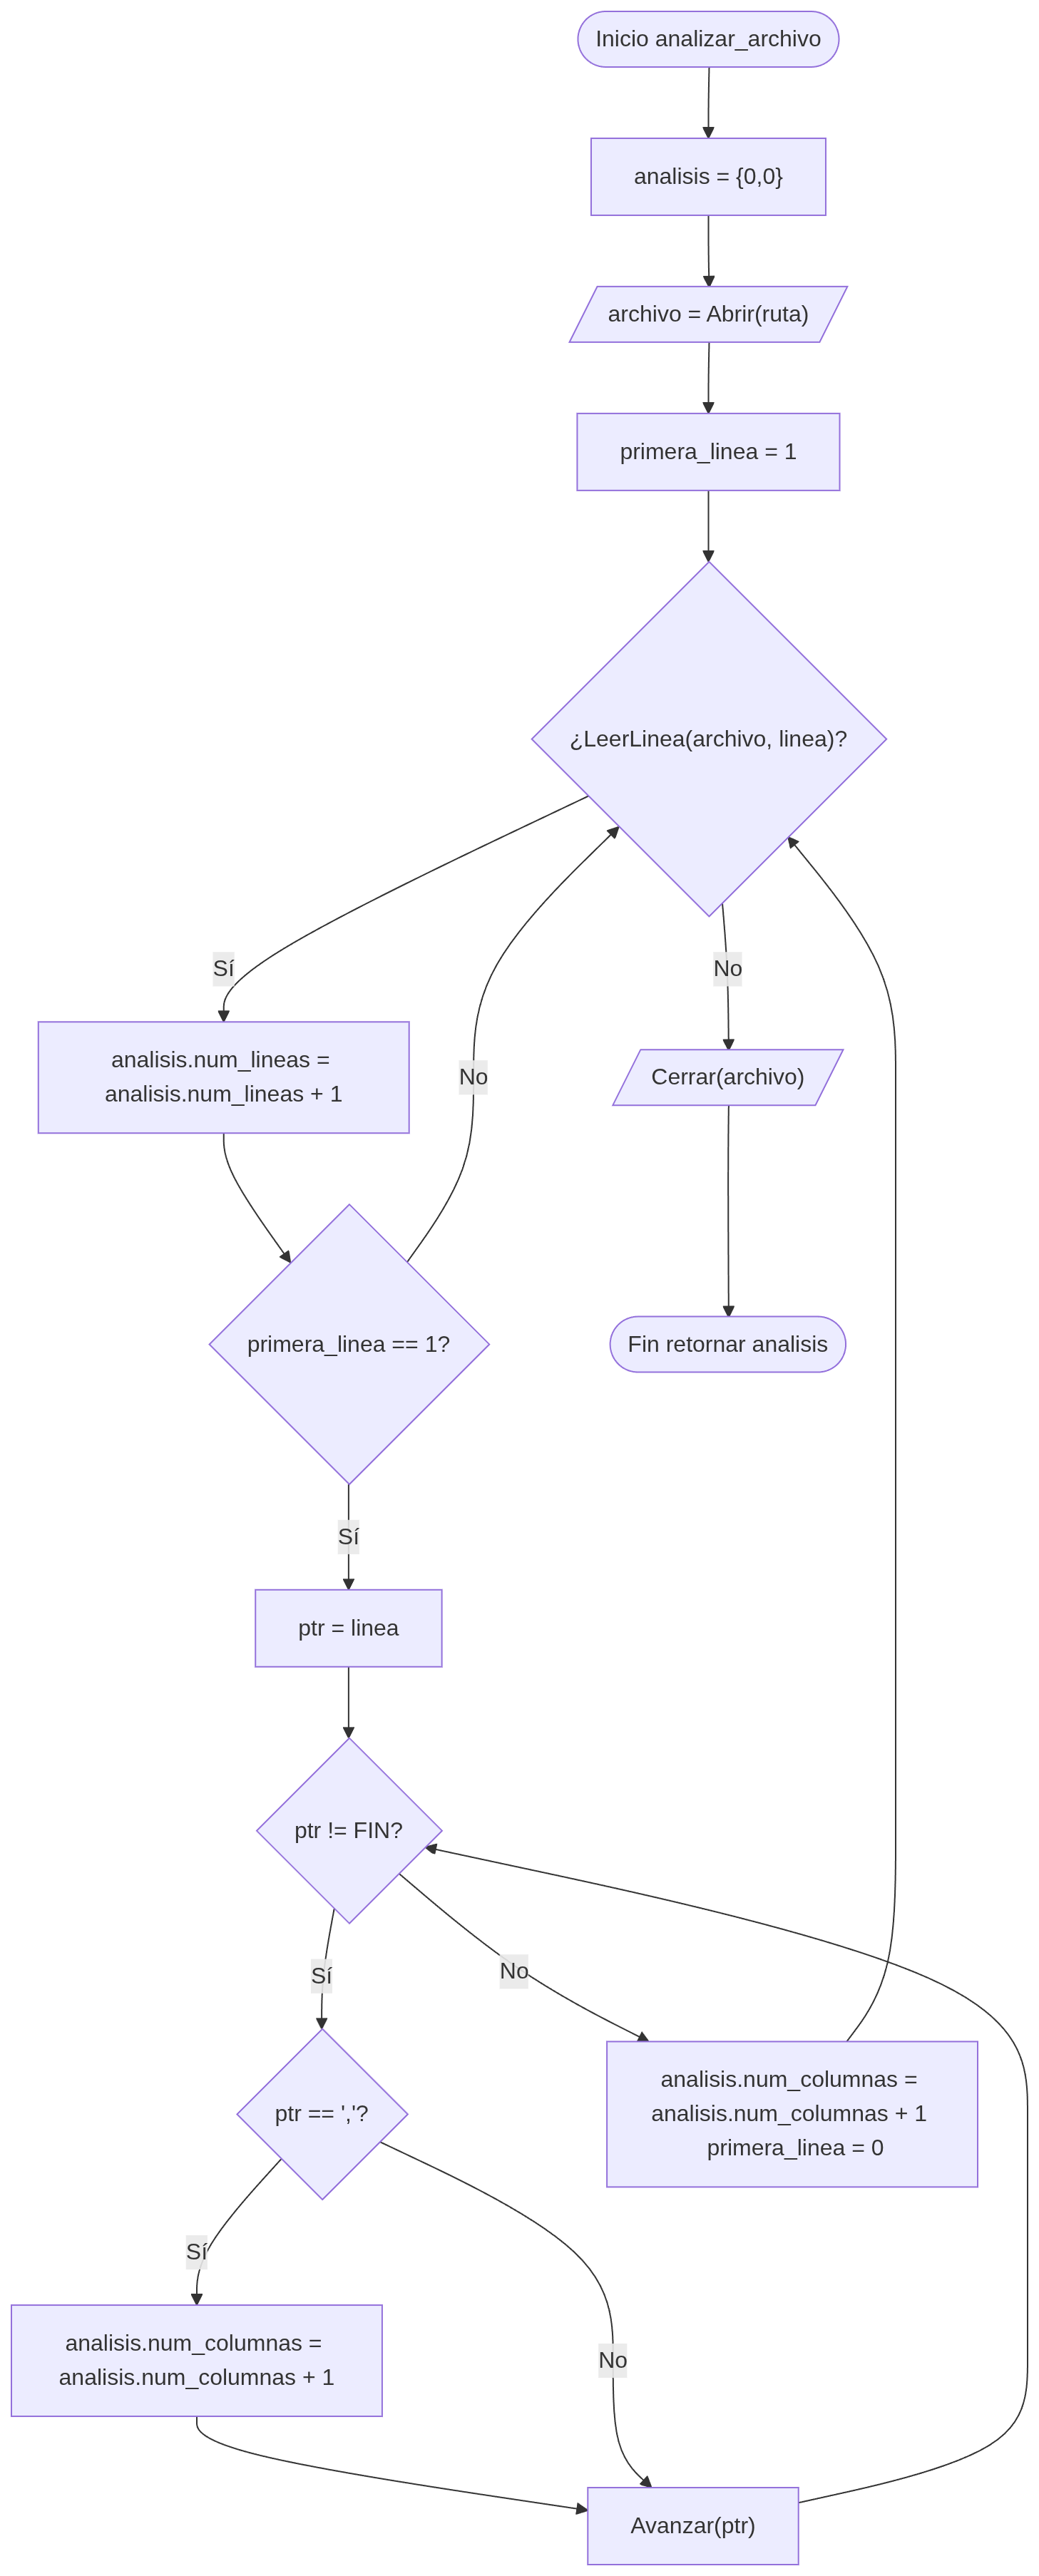
\includegraphics[width=0.45\textwidth]{funciones/analizar_archivo.png} 
    \caption{funciones.c/analizar\_archivo}
\end{figure}

\begin{figure}[H]
    \centering
    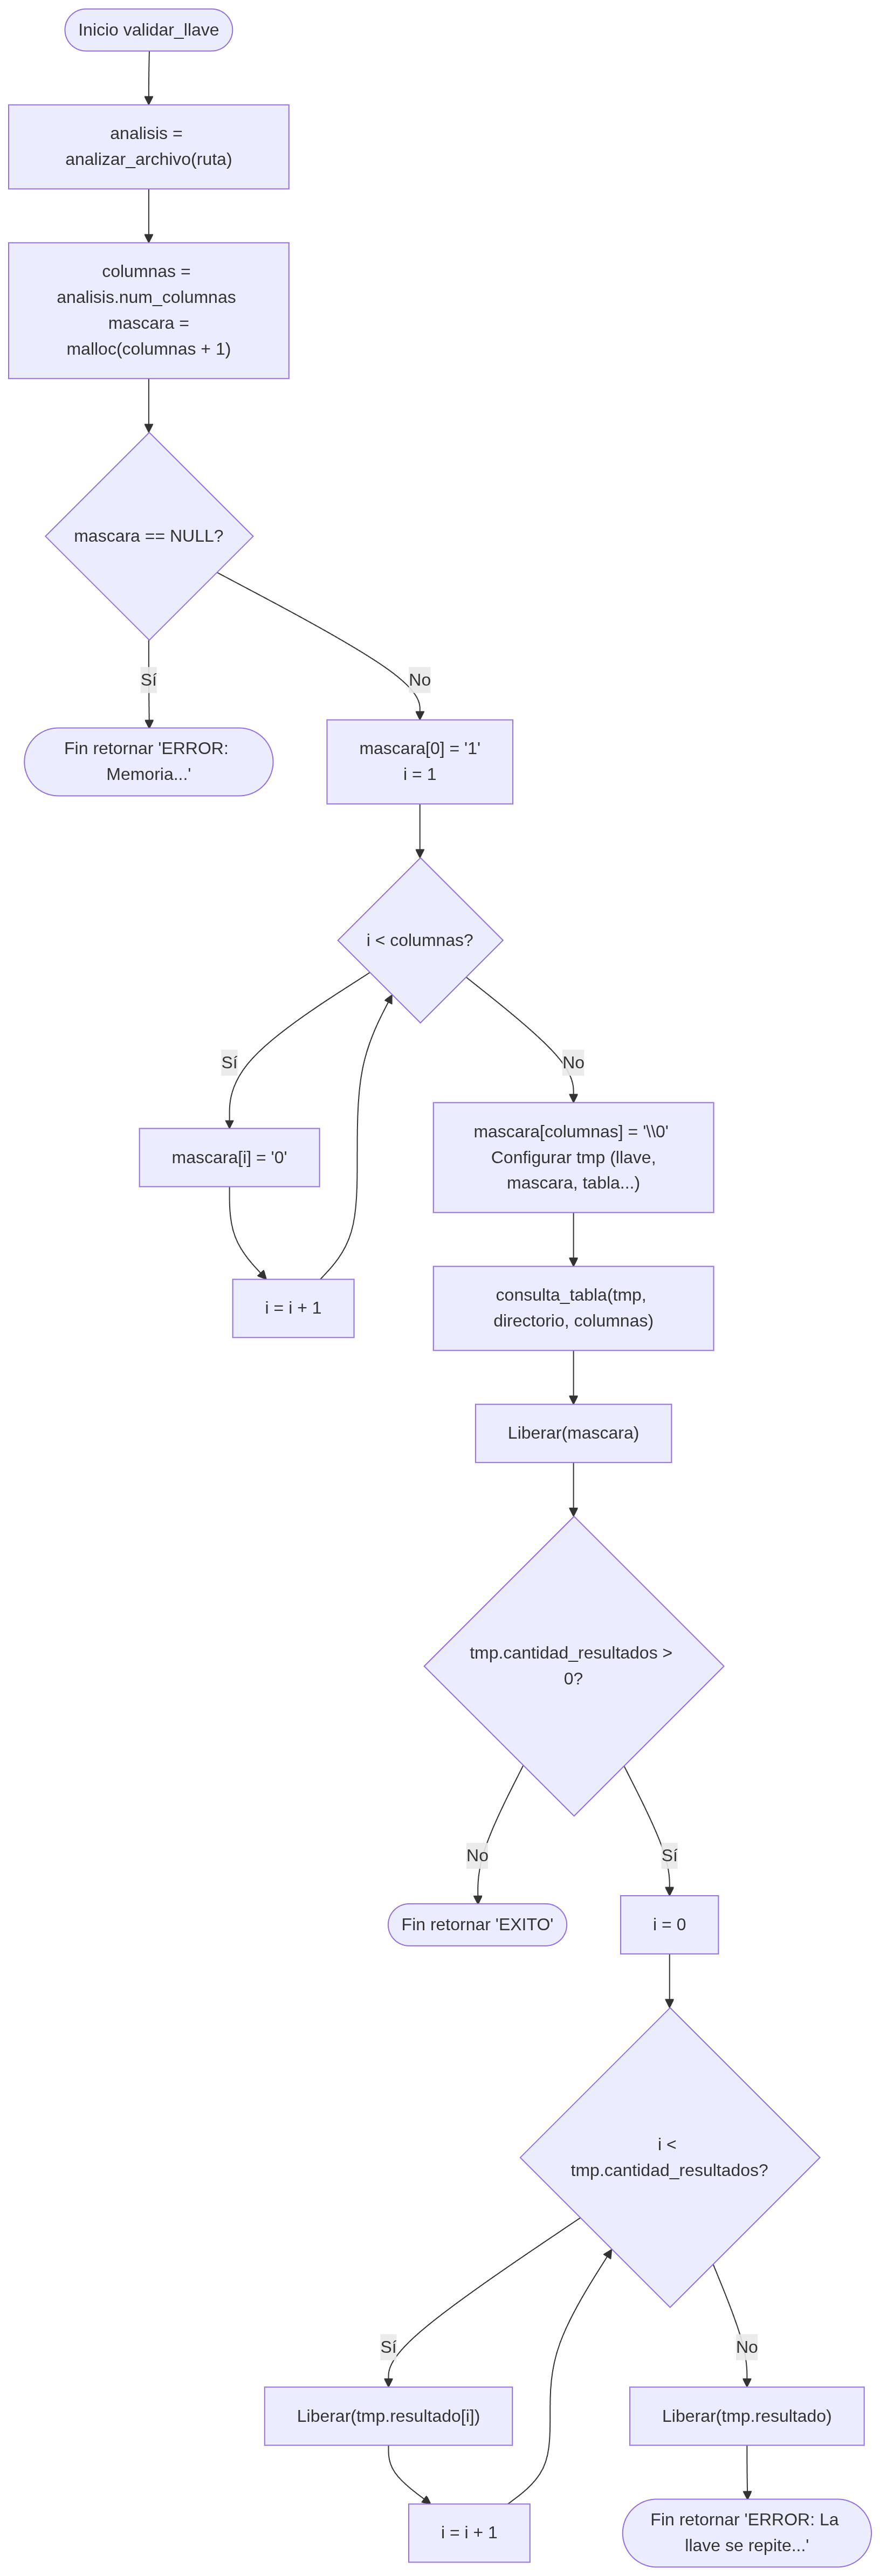
\includegraphics[width=0.4\textwidth]{funciones/validar_llave.png} 
    \caption{funciones.c/validar\_llave}
\end{figure}

\begin{figure}[H]
    \centering
    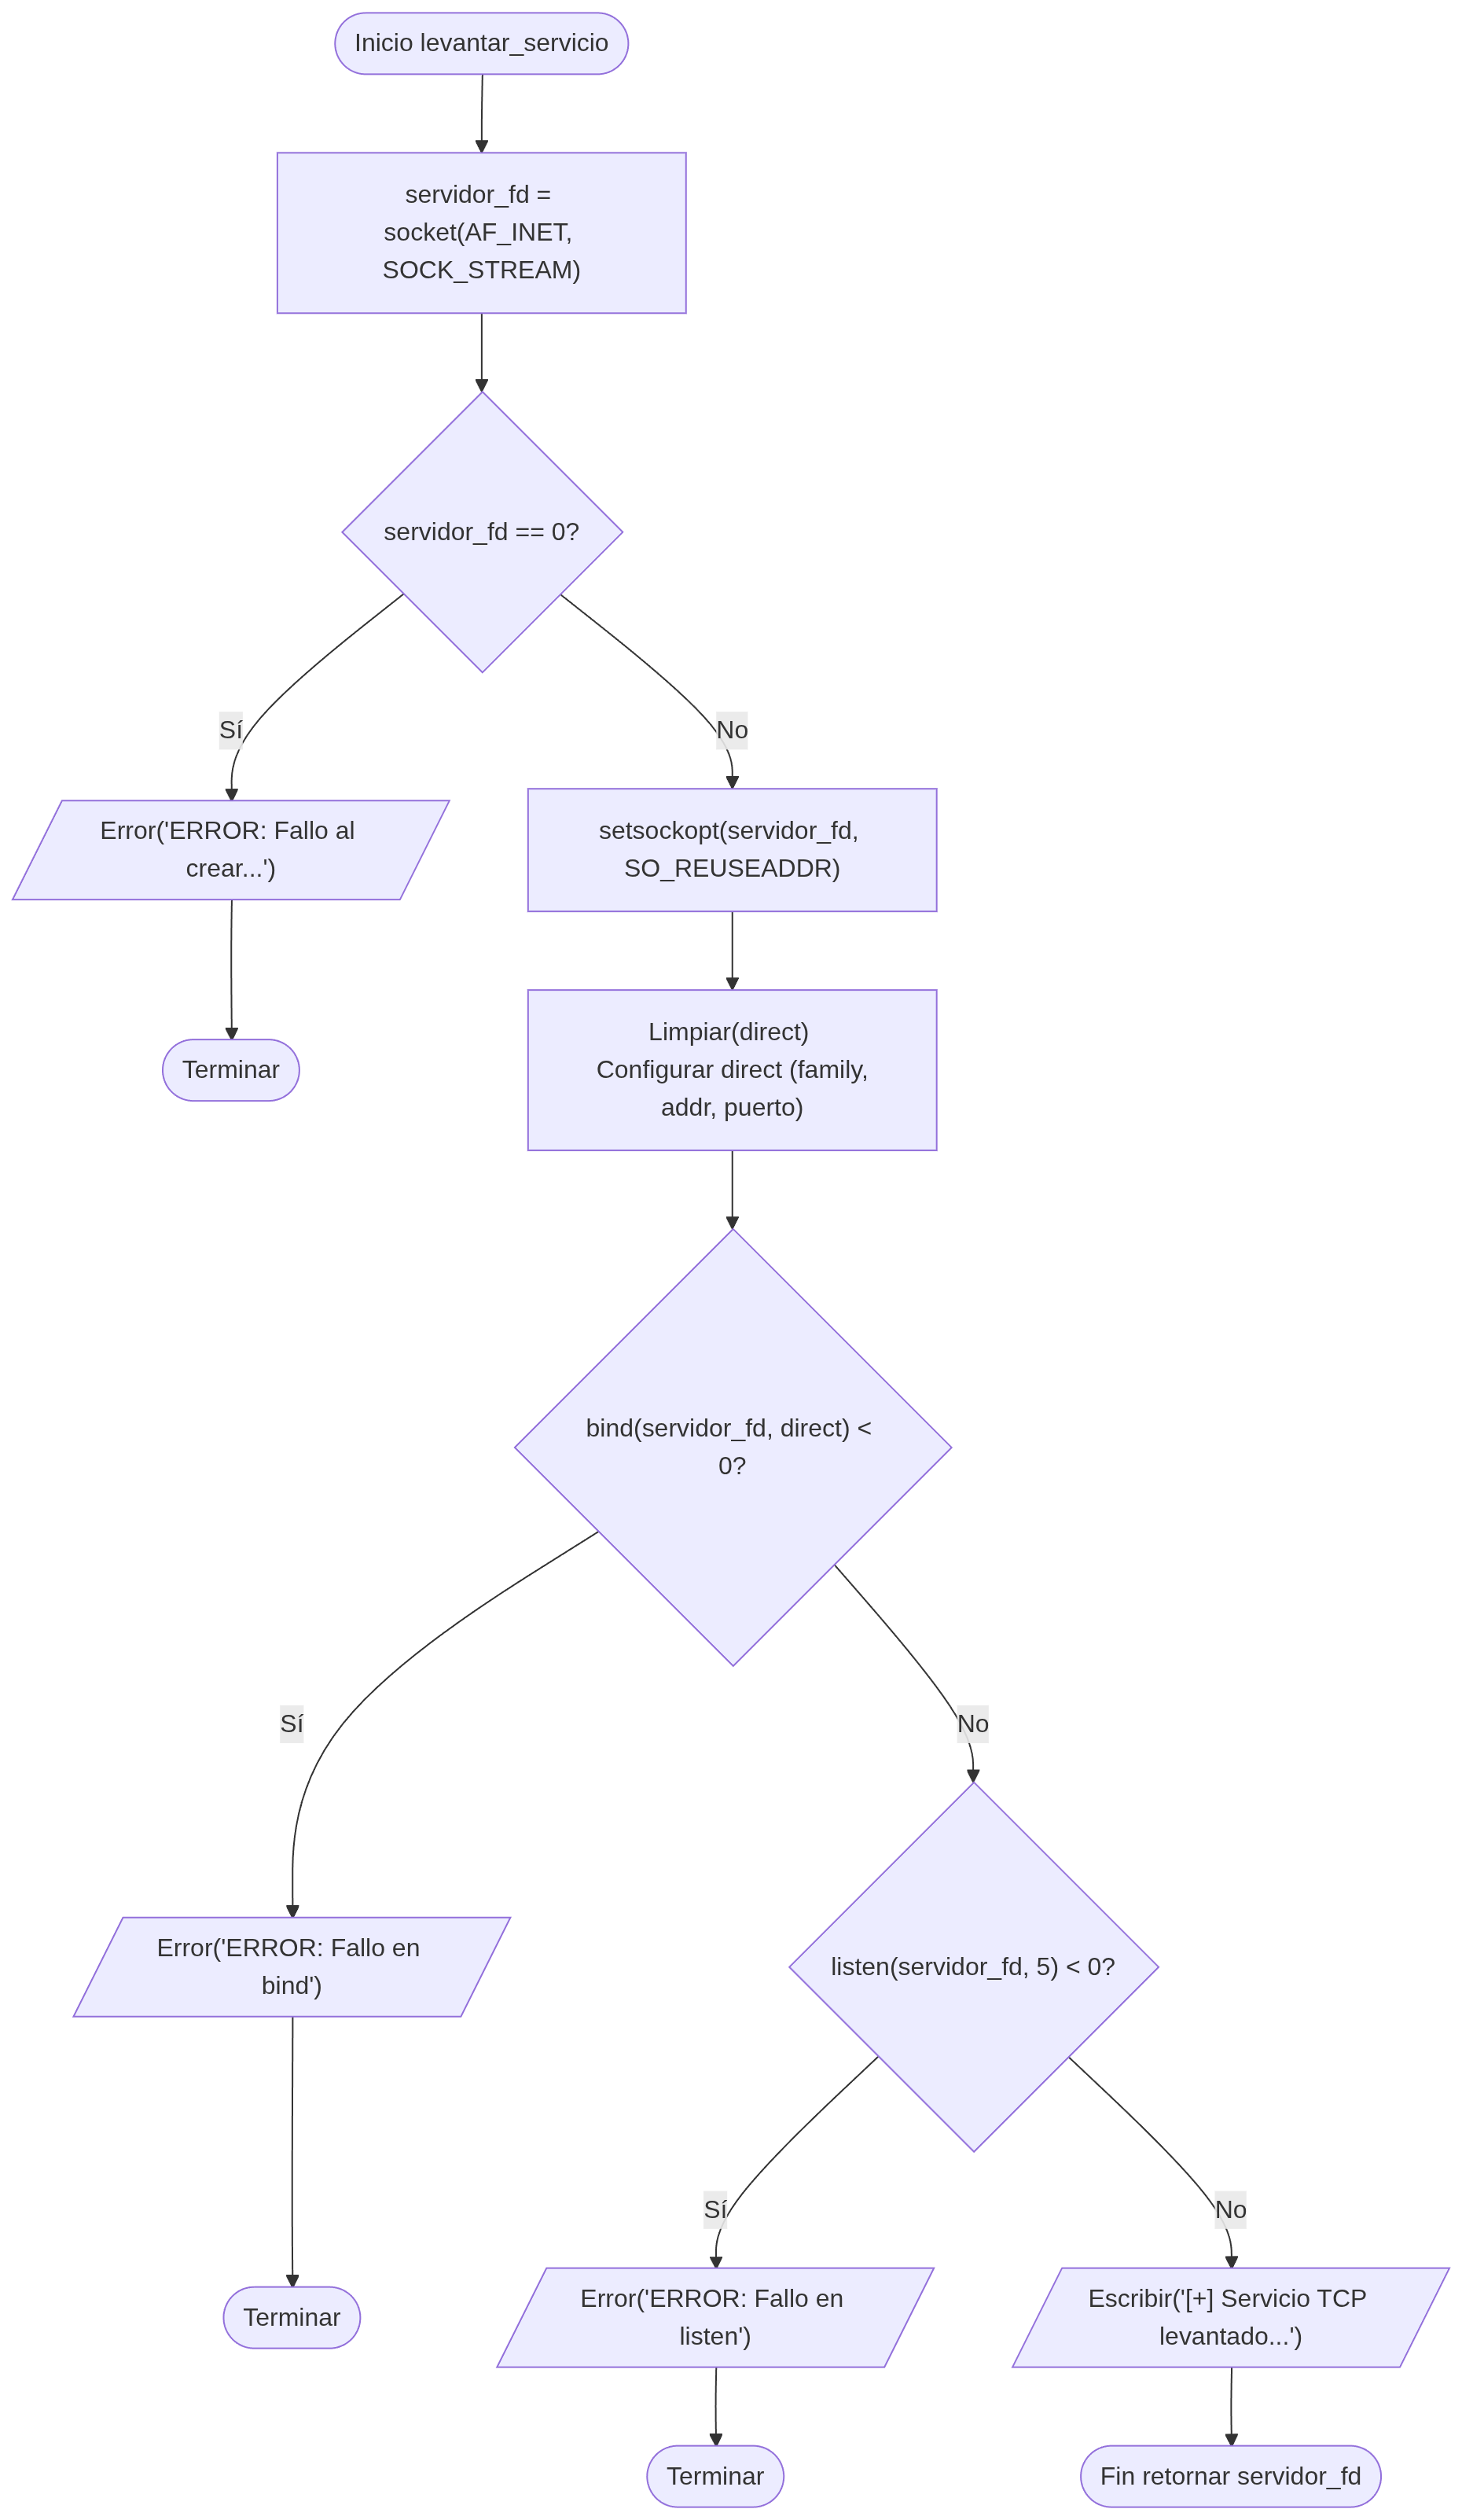
\includegraphics[width=0.6\textwidth]{funciones/levantar_servicio.png} 
    \caption{funciones.c/levantar\_servicio}
\end{figure}

\begin{itemize}
    \item \textbf{Diagrama de Flujo (consultas.c)}
\end{itemize}

\setcounter{figure}{0} % La siguiente figura será la número 1

\begin{figure}[H]
    \centering
    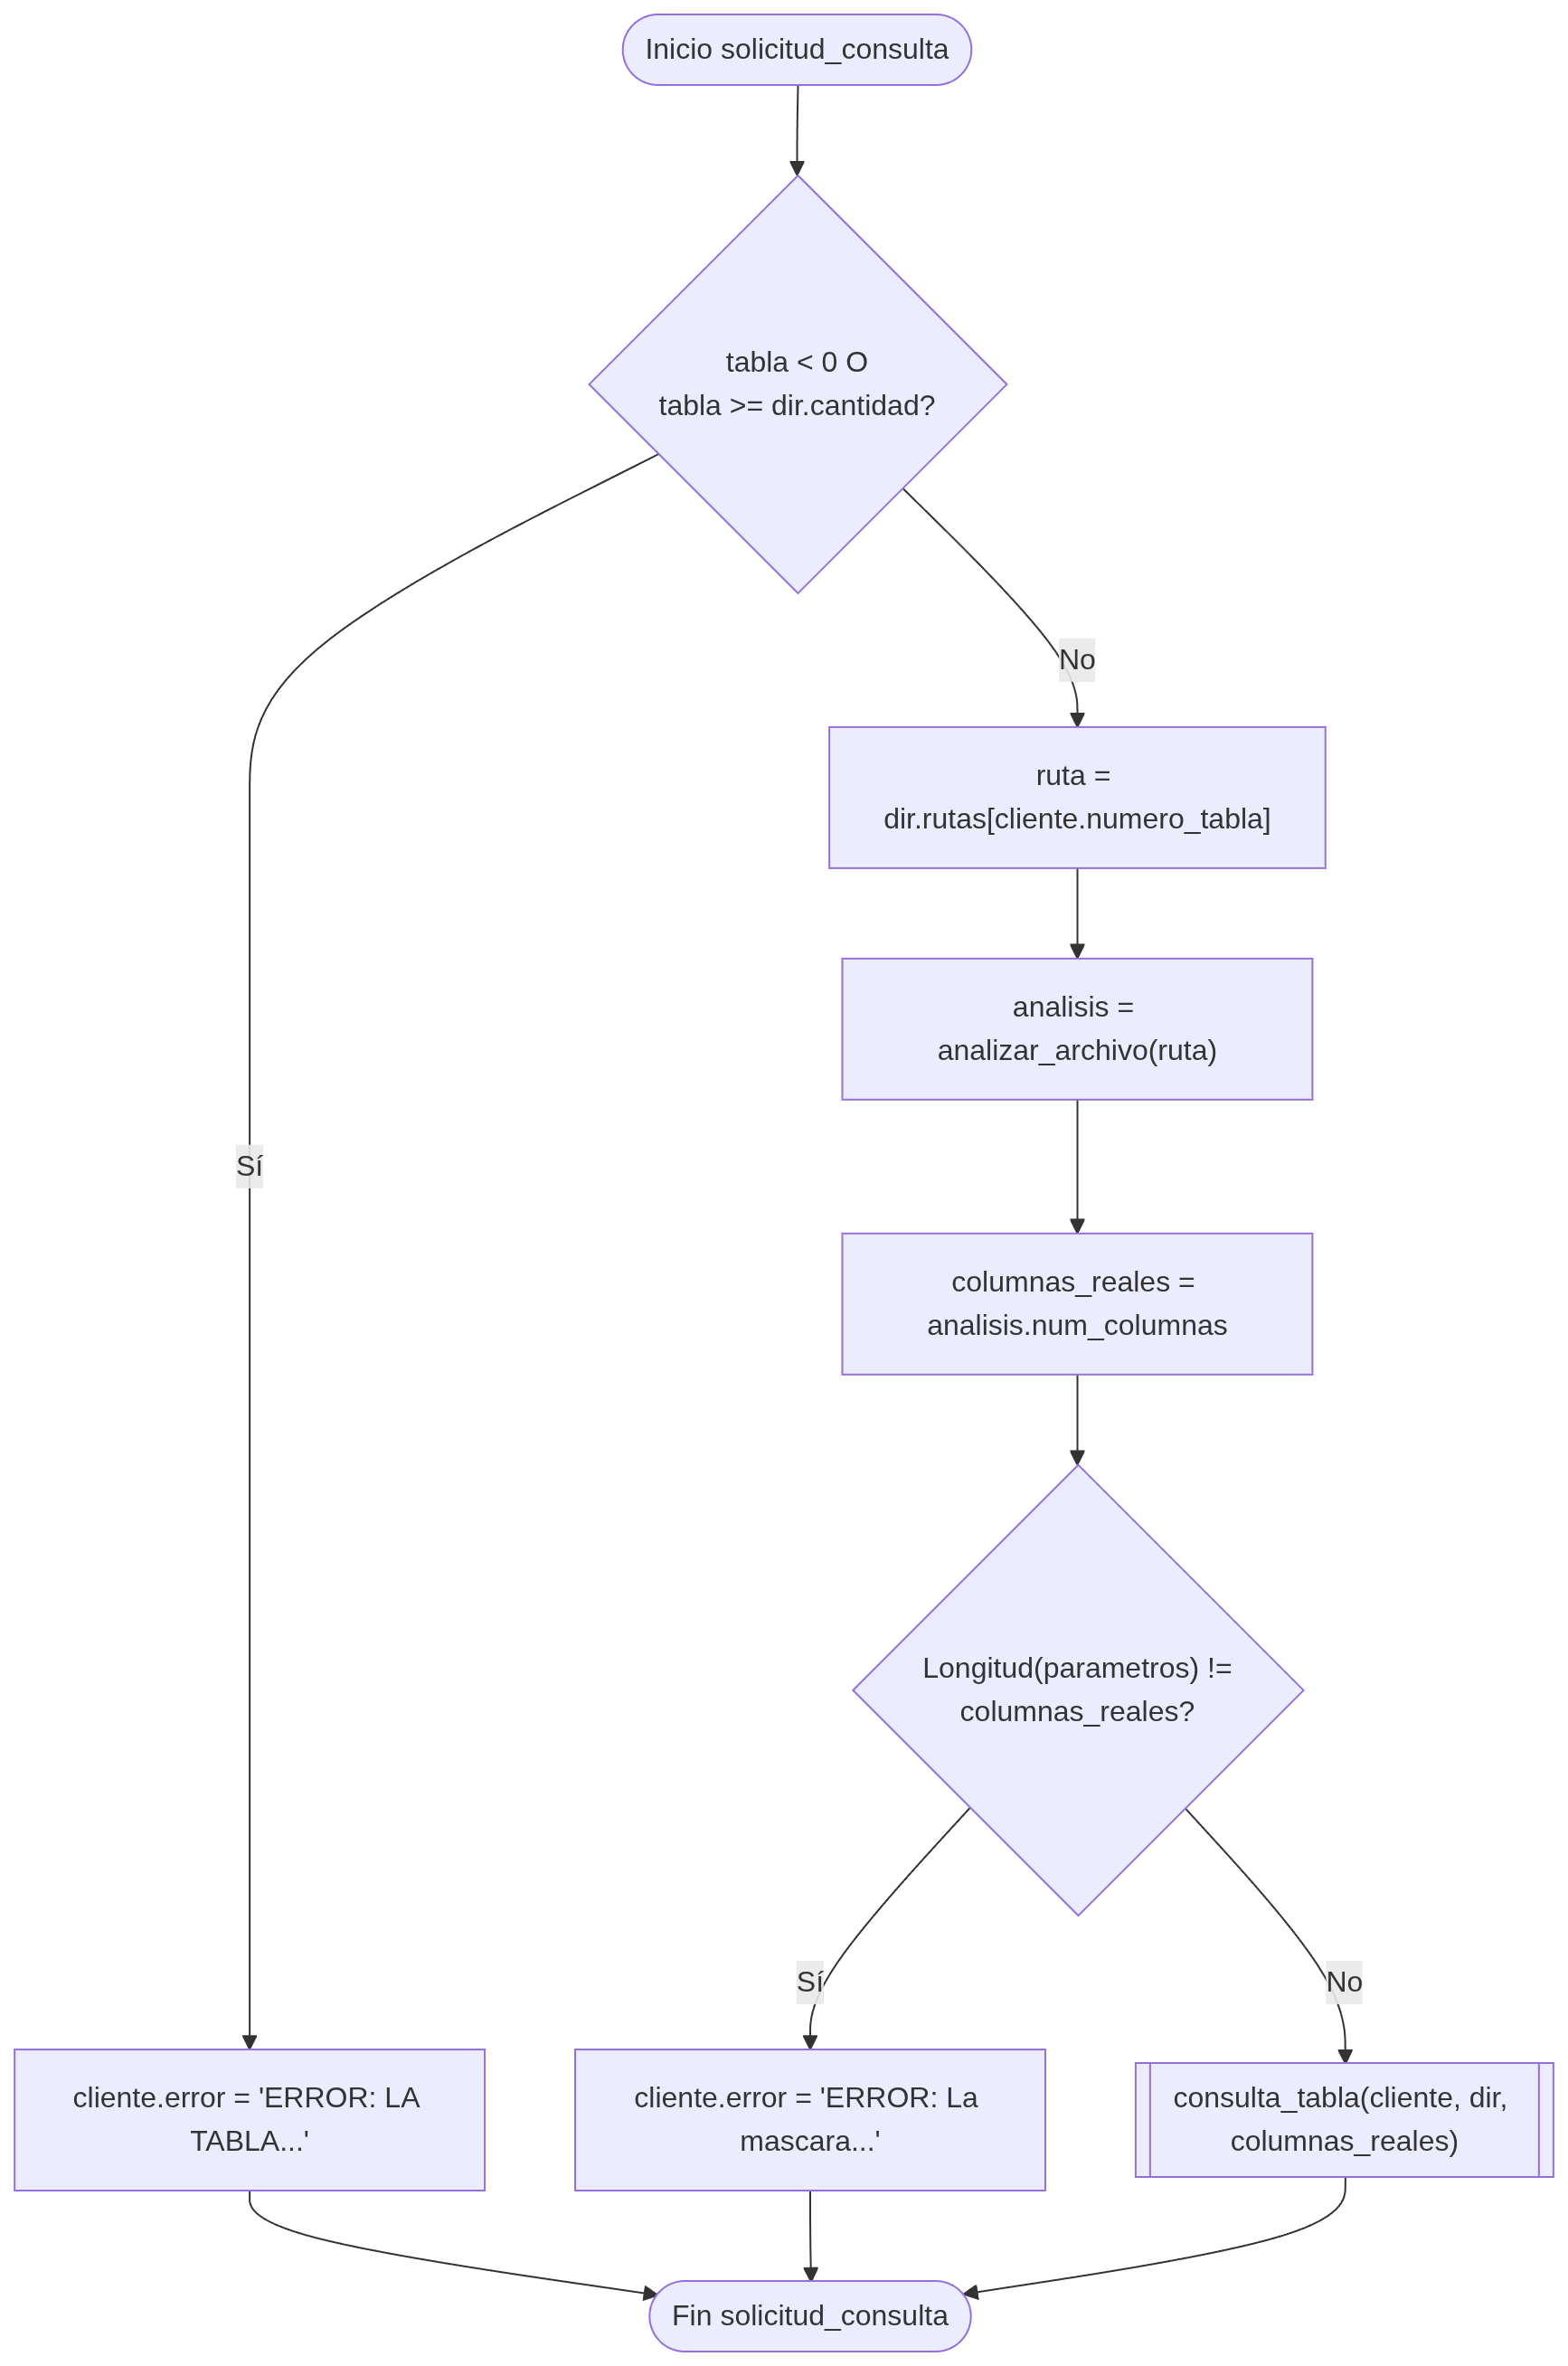
\includegraphics[width=0.6\textwidth]{consulta/solicitud_consulta.png} 
    \caption{consulta.c/solicitud\_consulta}
\end{figure}

\begin{figure}[H]
    \centering
    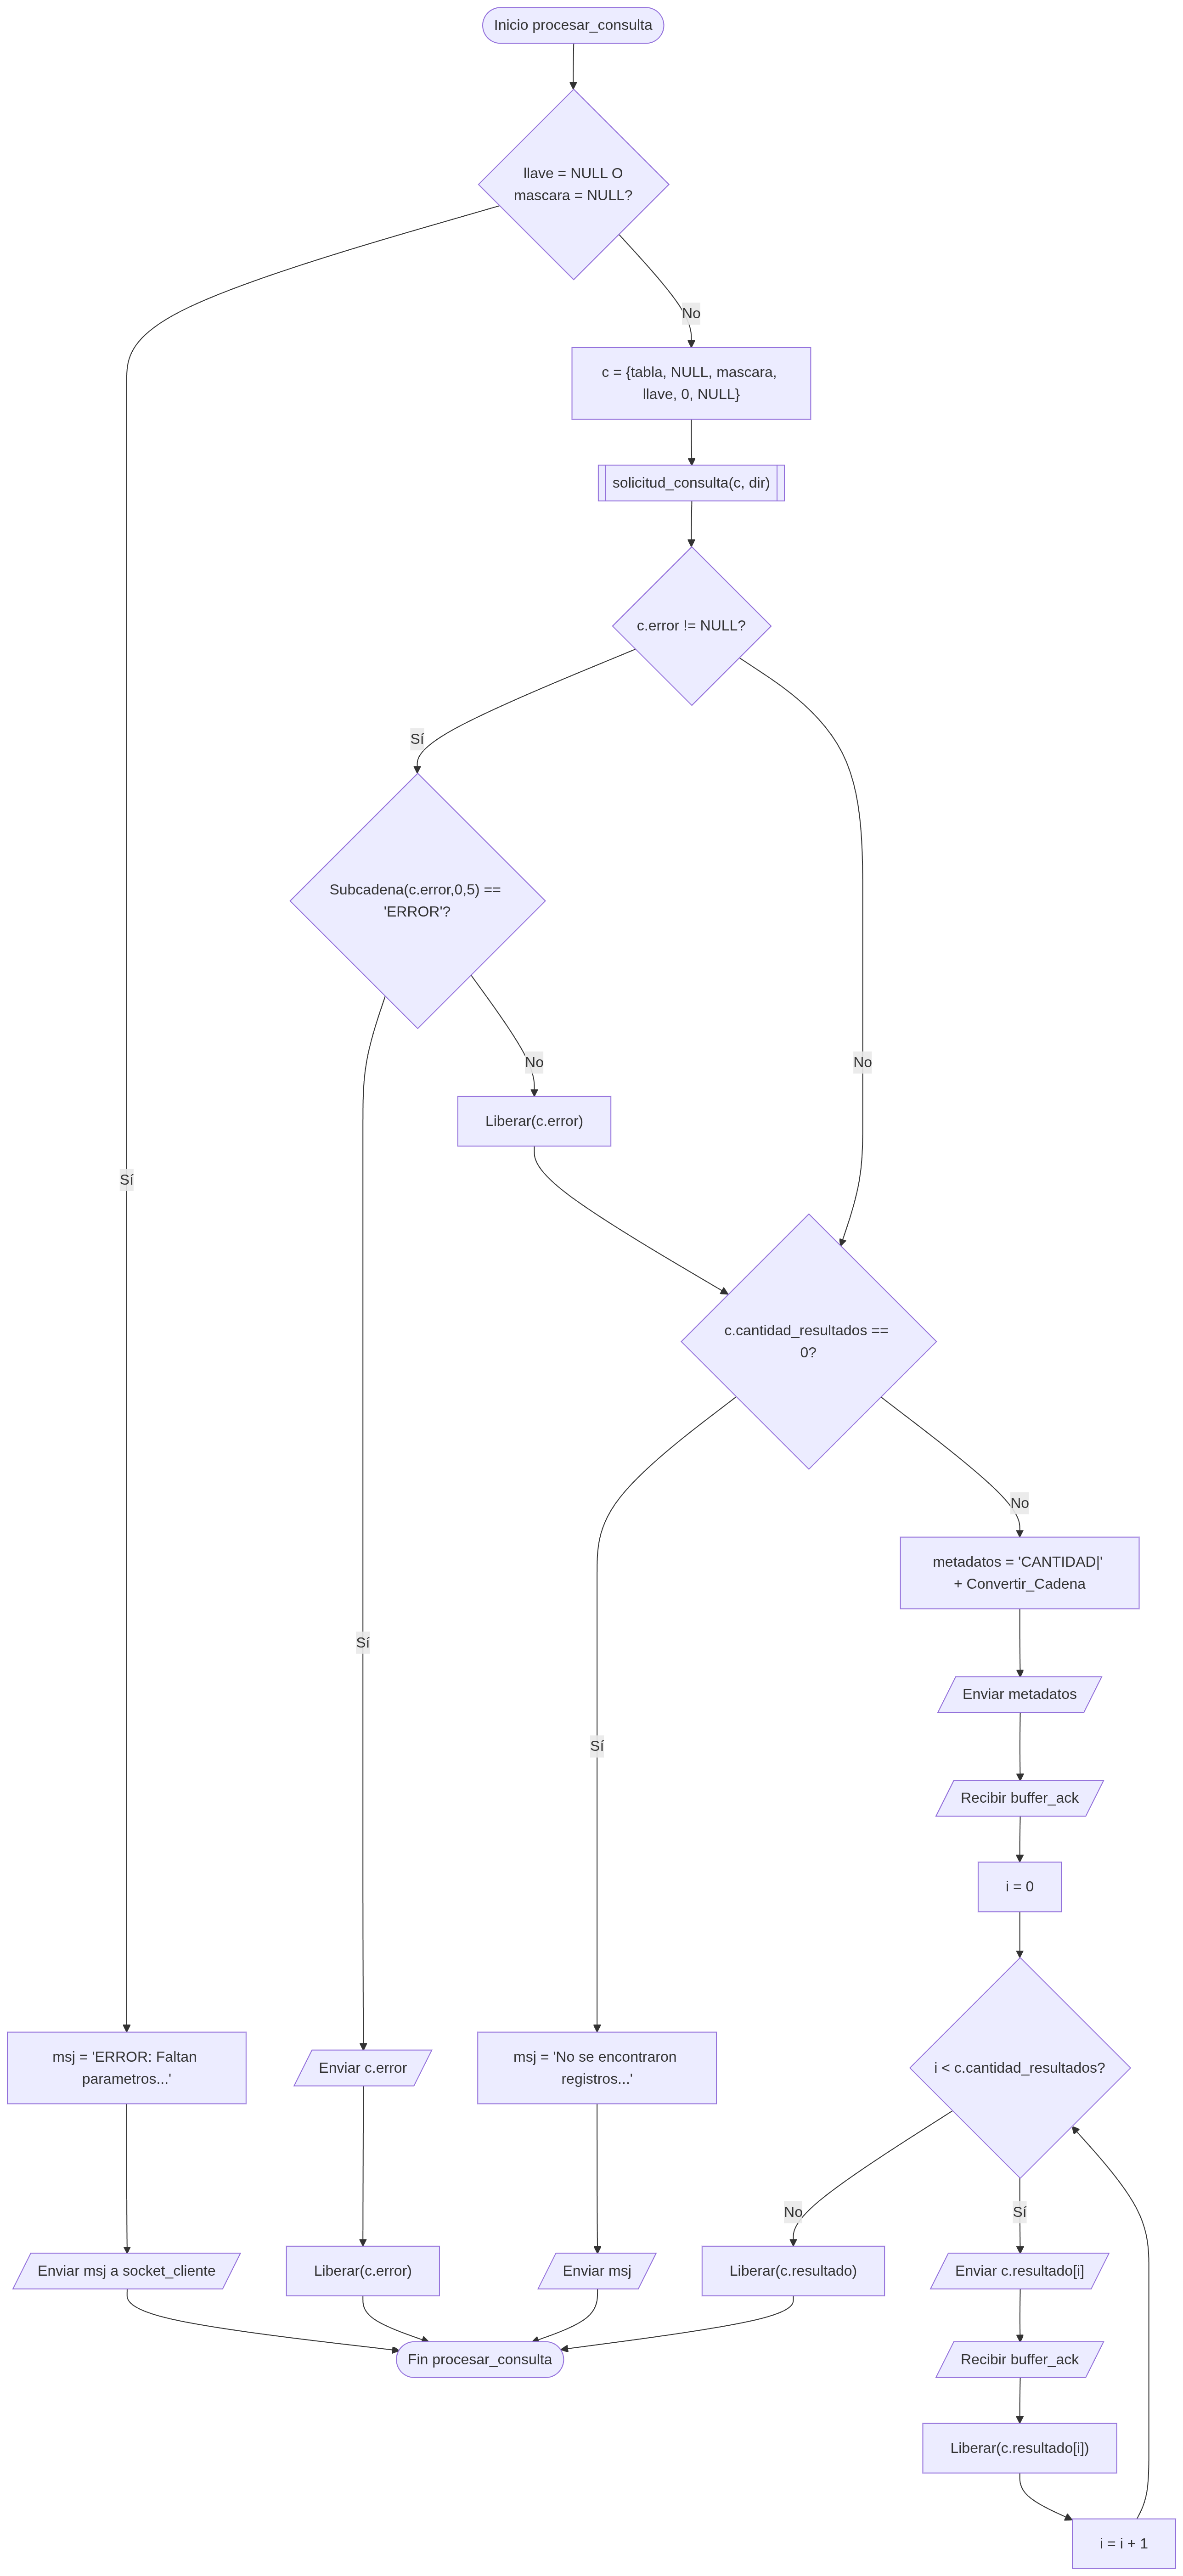
\includegraphics[width=0.5\textwidth]{consulta/procesar_consulta.png} 
    \caption{consulta.c/procesar\_consulta}
\end{figure}

\begin{figure}[H]
    \centering
    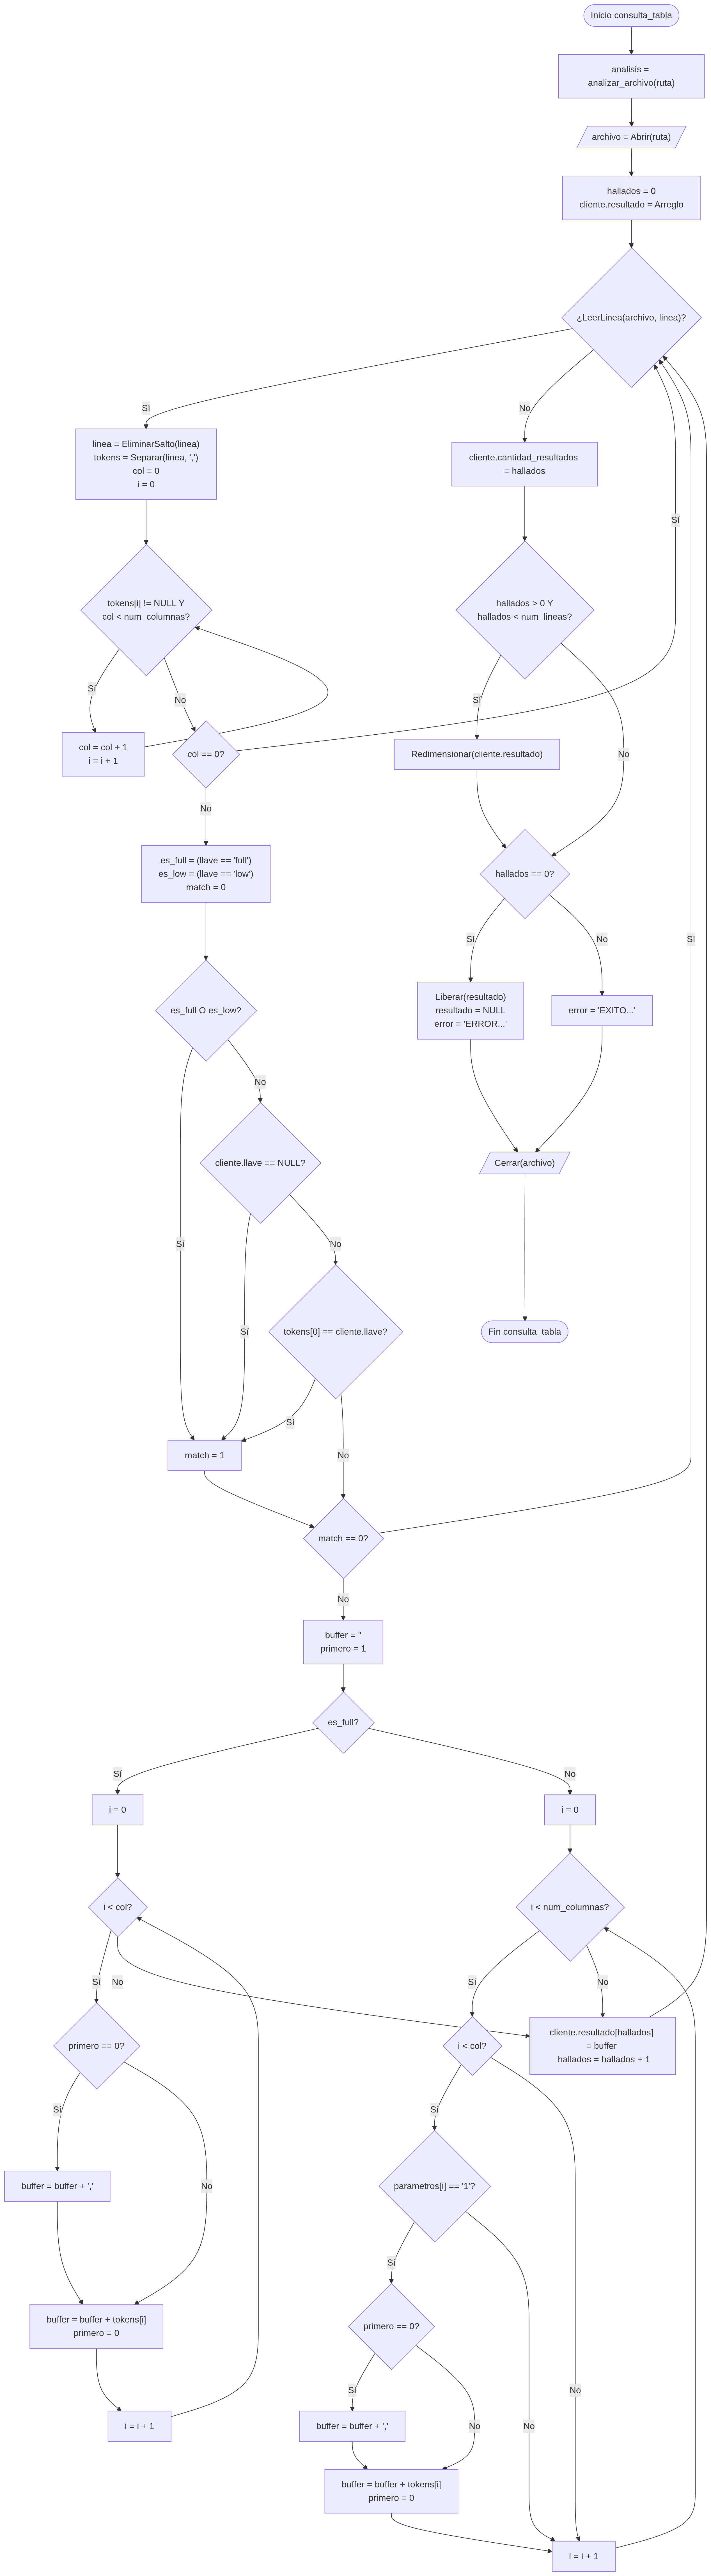
\includegraphics[width=0.3\textwidth]{consulta/consulta_tabla.png} 
    \caption{consulta.c/consulta\_tabla}
\end{figure}

\begin{itemize}
    \item \textbf{Diagrama de Flujo (insercion.c)}
\end{itemize}

\setcounter{figure}{0} % La siguiente figura será la número 1

\begin{figure}[H]
    \centering
    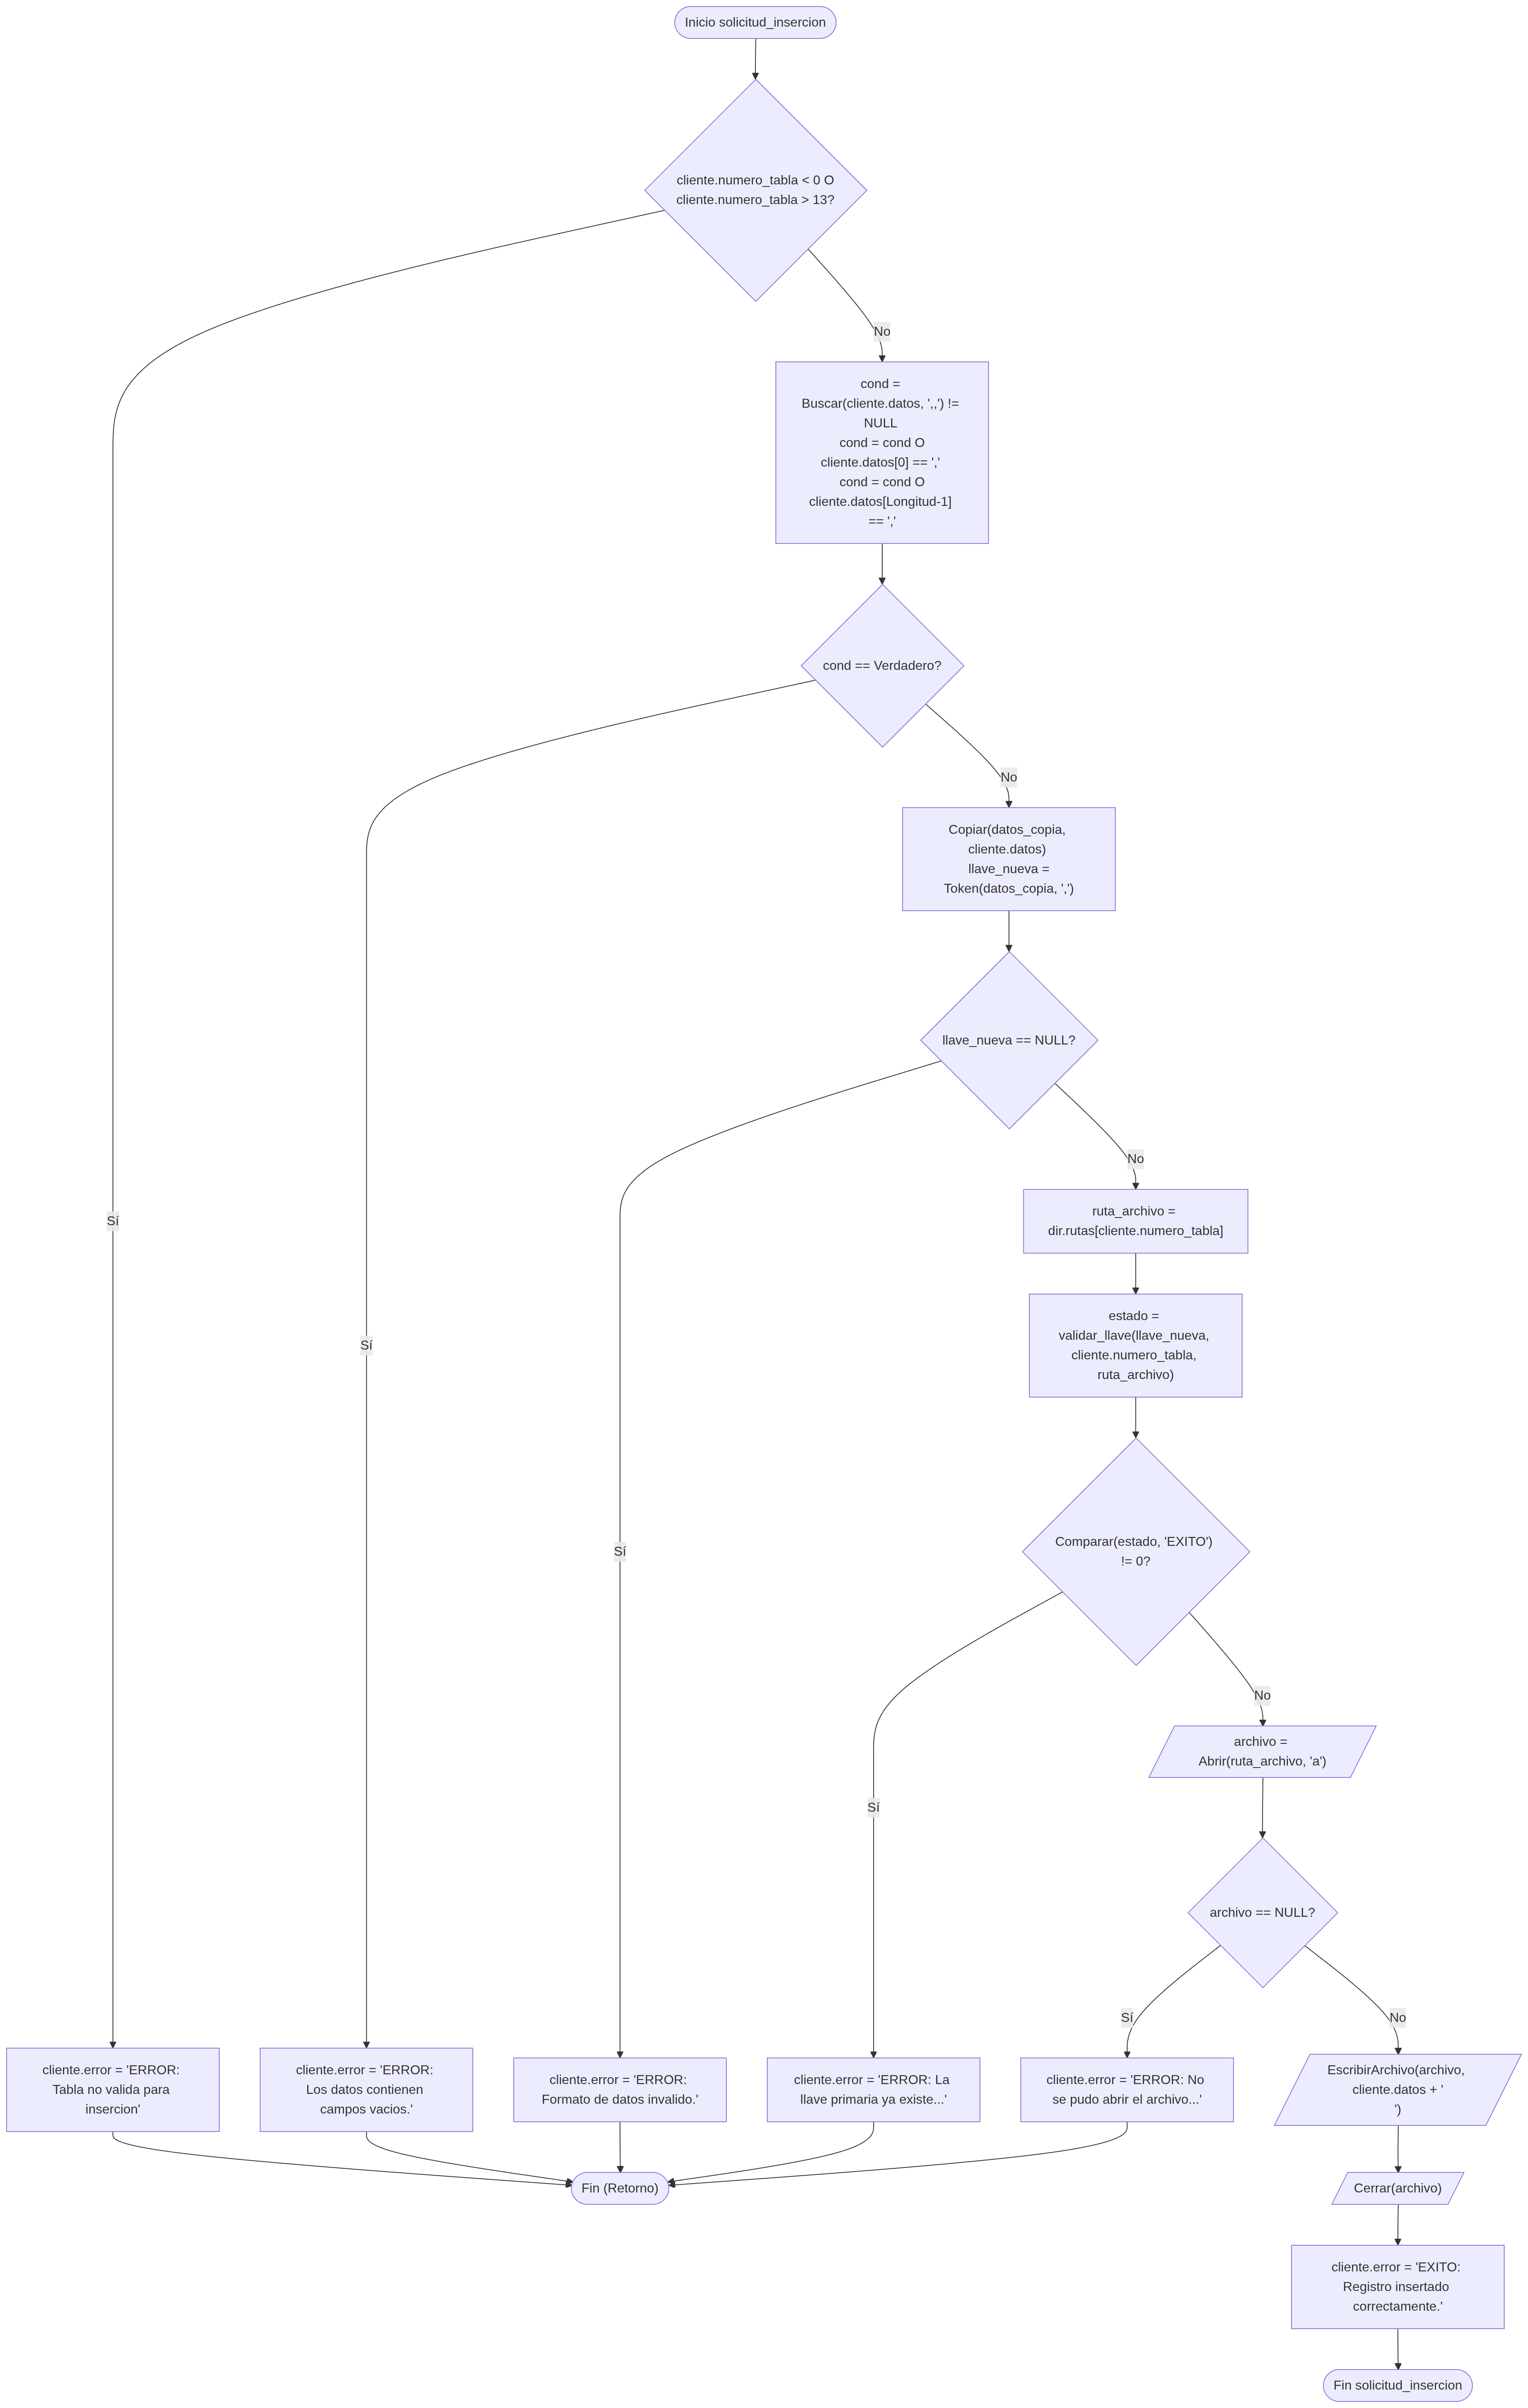
\includegraphics[width=0.65\textwidth]{insercion/solicitud_insercion.png} 
    \caption{insercion.c/solicitud\_insercion}
\end{figure}

\begin{figure}[H]
    \centering
    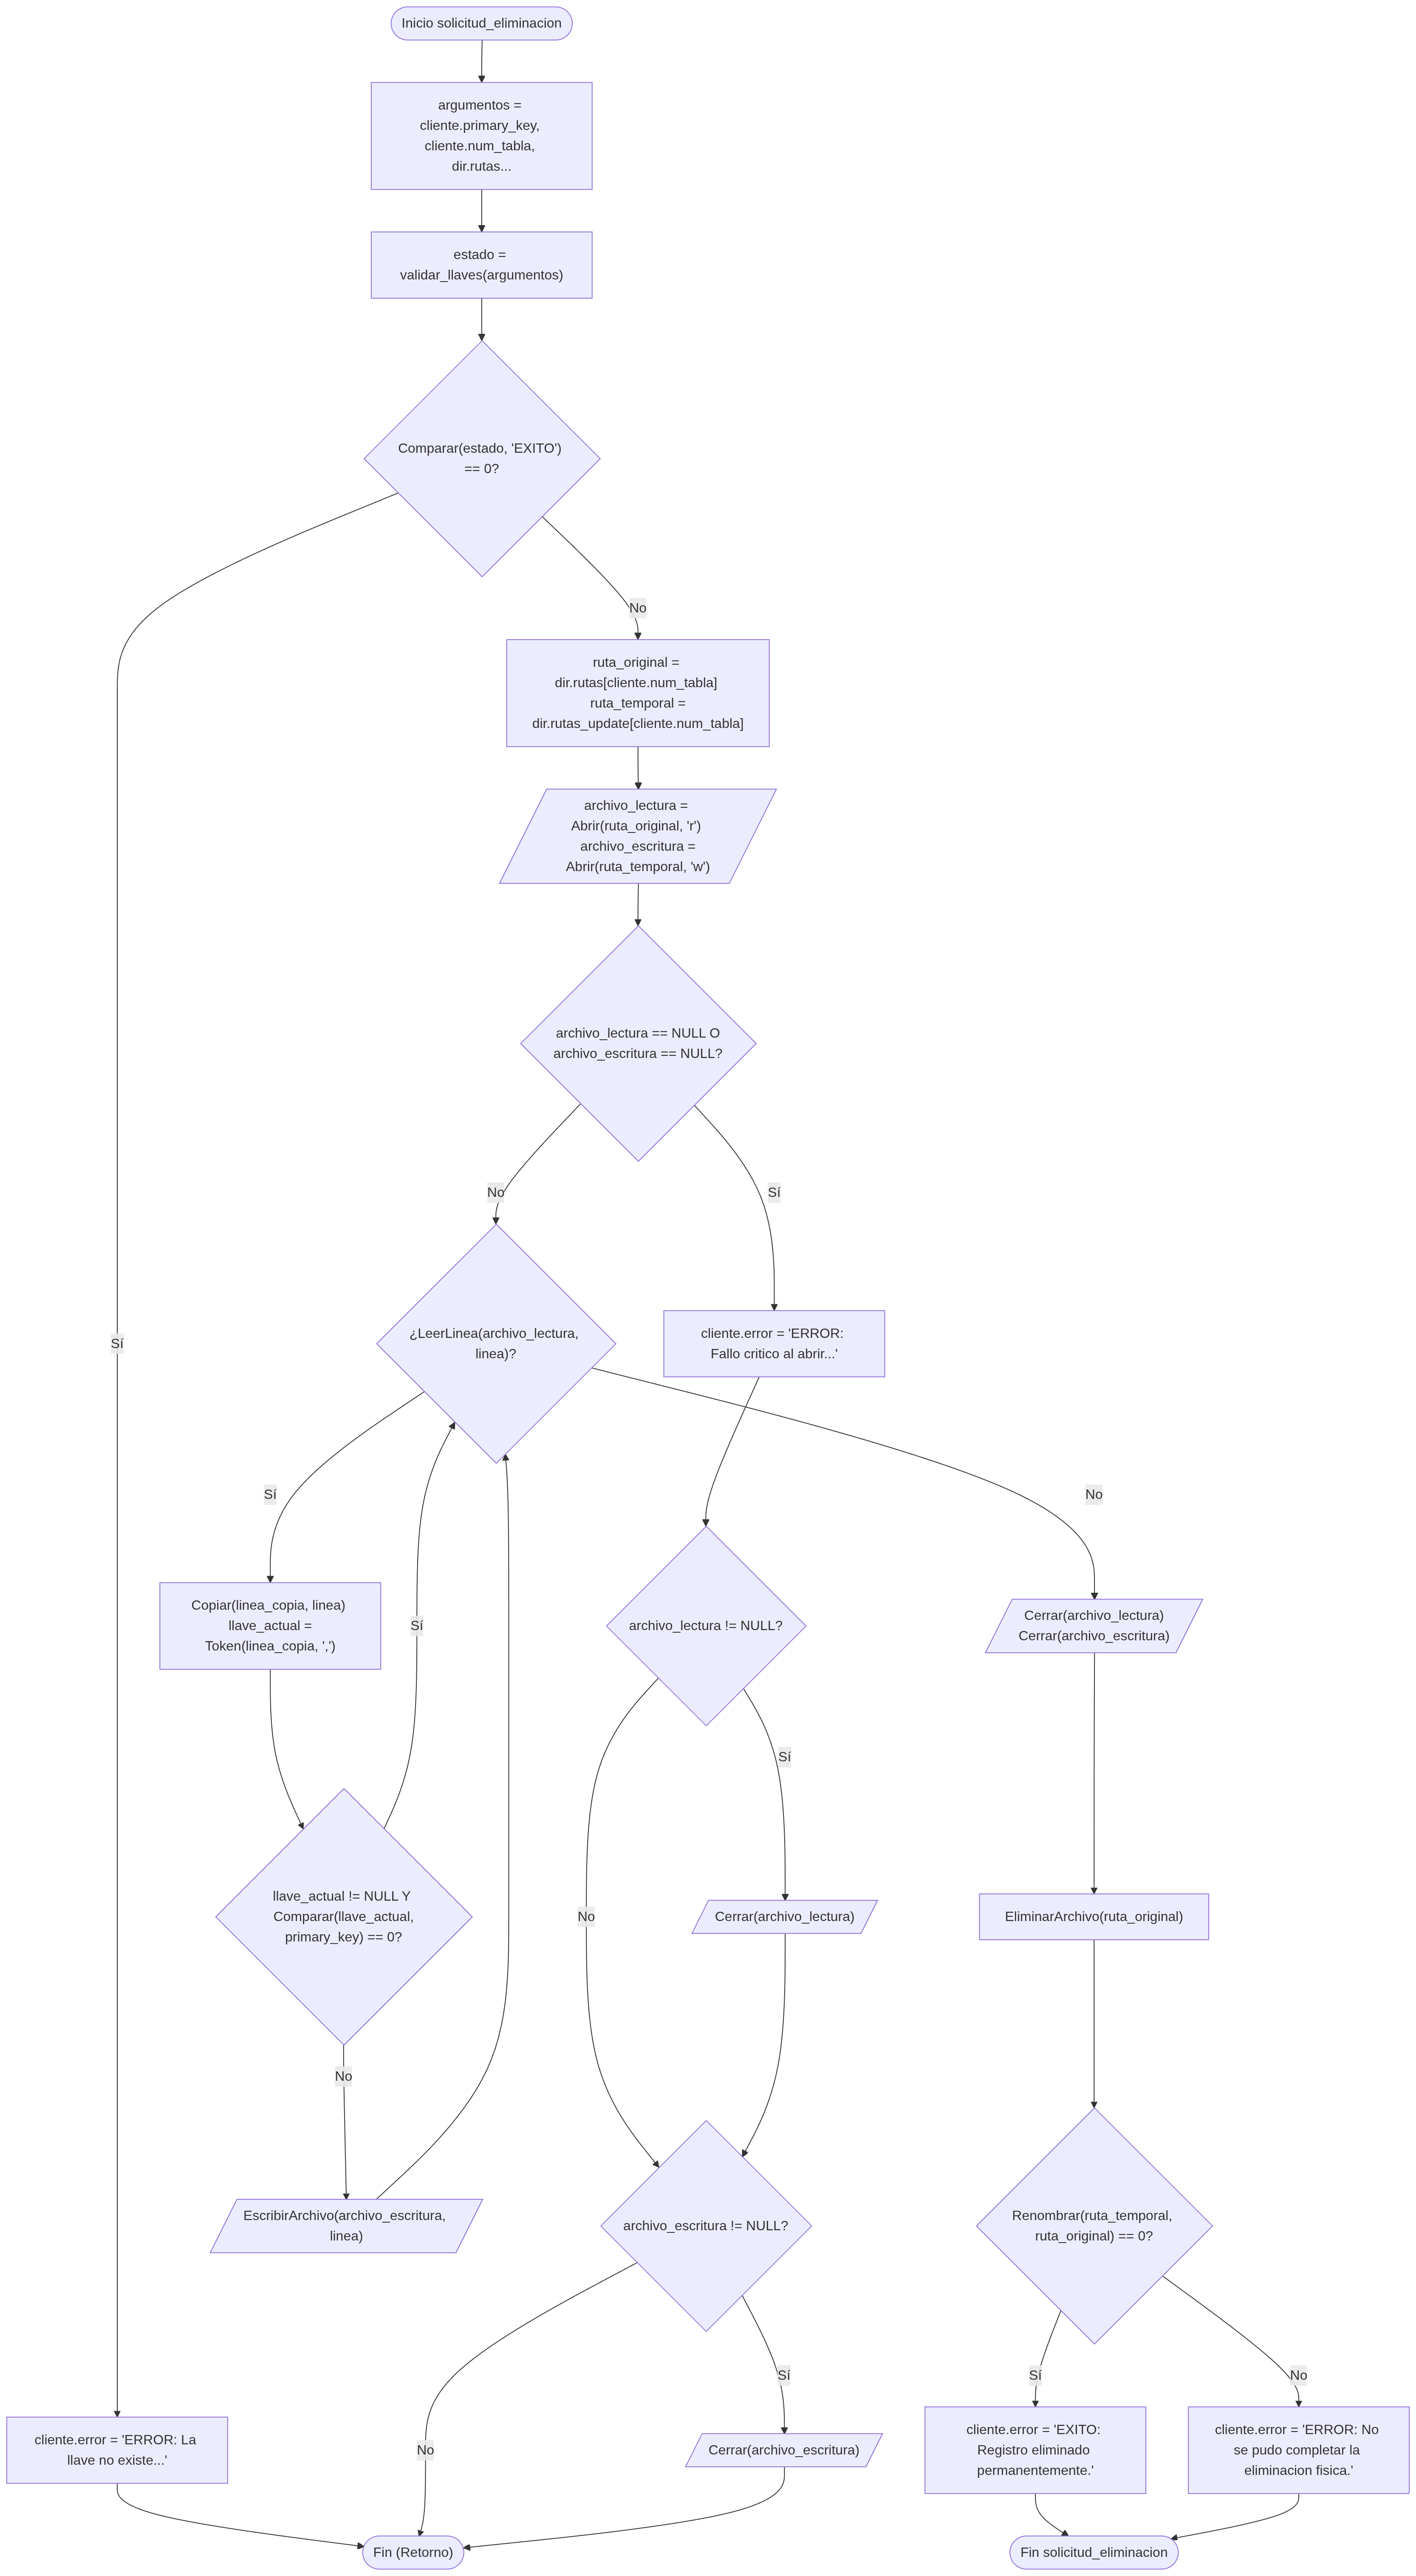
\includegraphics[width=0.65\textwidth]{insercion/solicitud_eliminacion.png} 
    \caption{insercion.c/solicitud\_eliminacion}
\end{figure}

\begin{itemize}
    \item \textbf{Diagrama de Flujo (update.c)}
\end{itemize}

\setcounter{figure}{0} % La siguiente figura será la número 1

\begin{figure}[H]
    \centering
    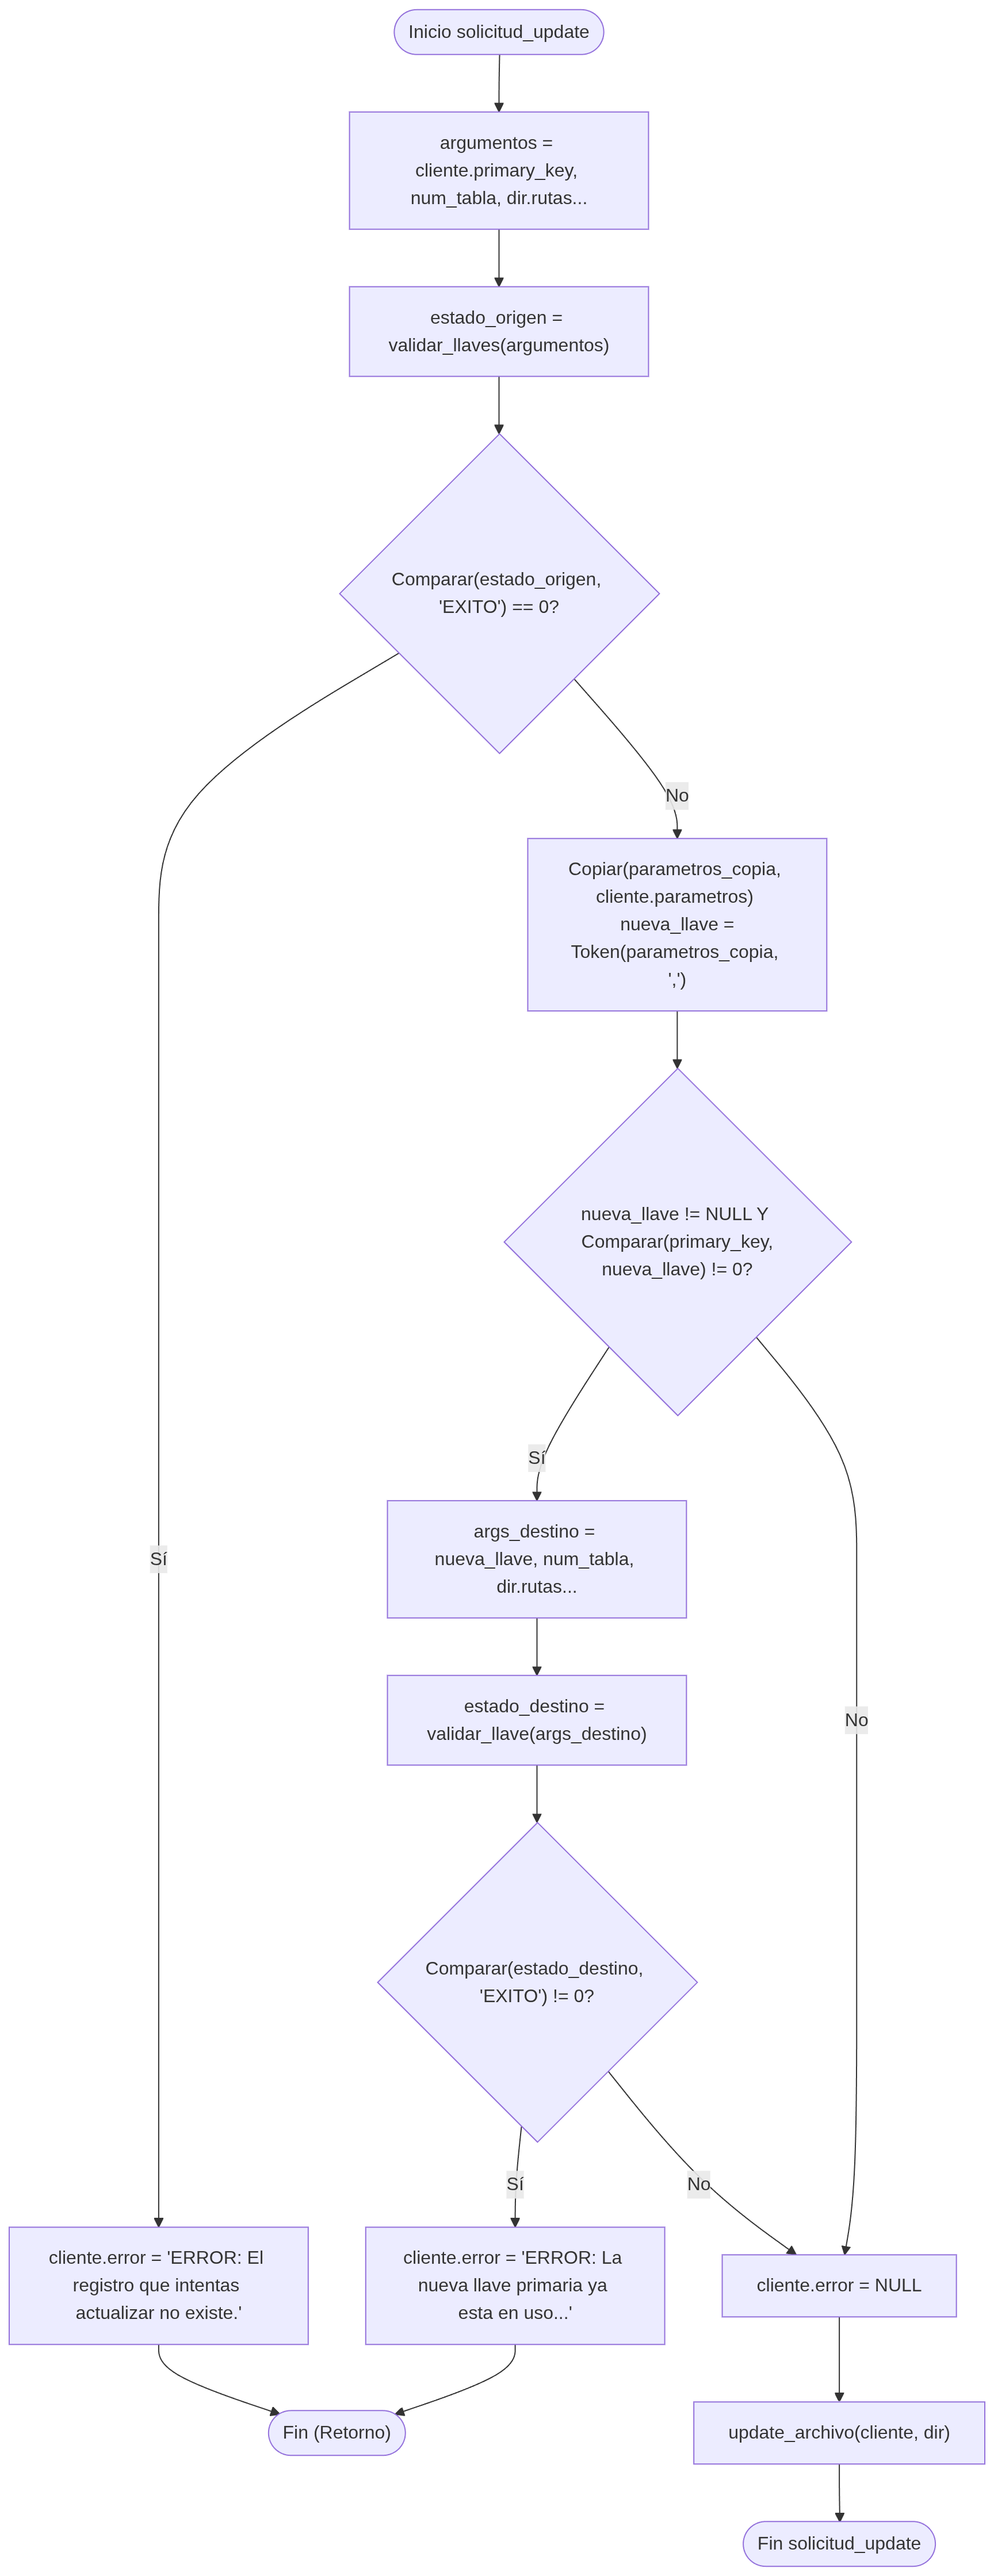
\includegraphics[width=0.4\textwidth]{update/solicitud_update.png} 
    \caption{update.c/solicitud\_update}
\end{figure}

\begin{figure}[H]
    \centering
    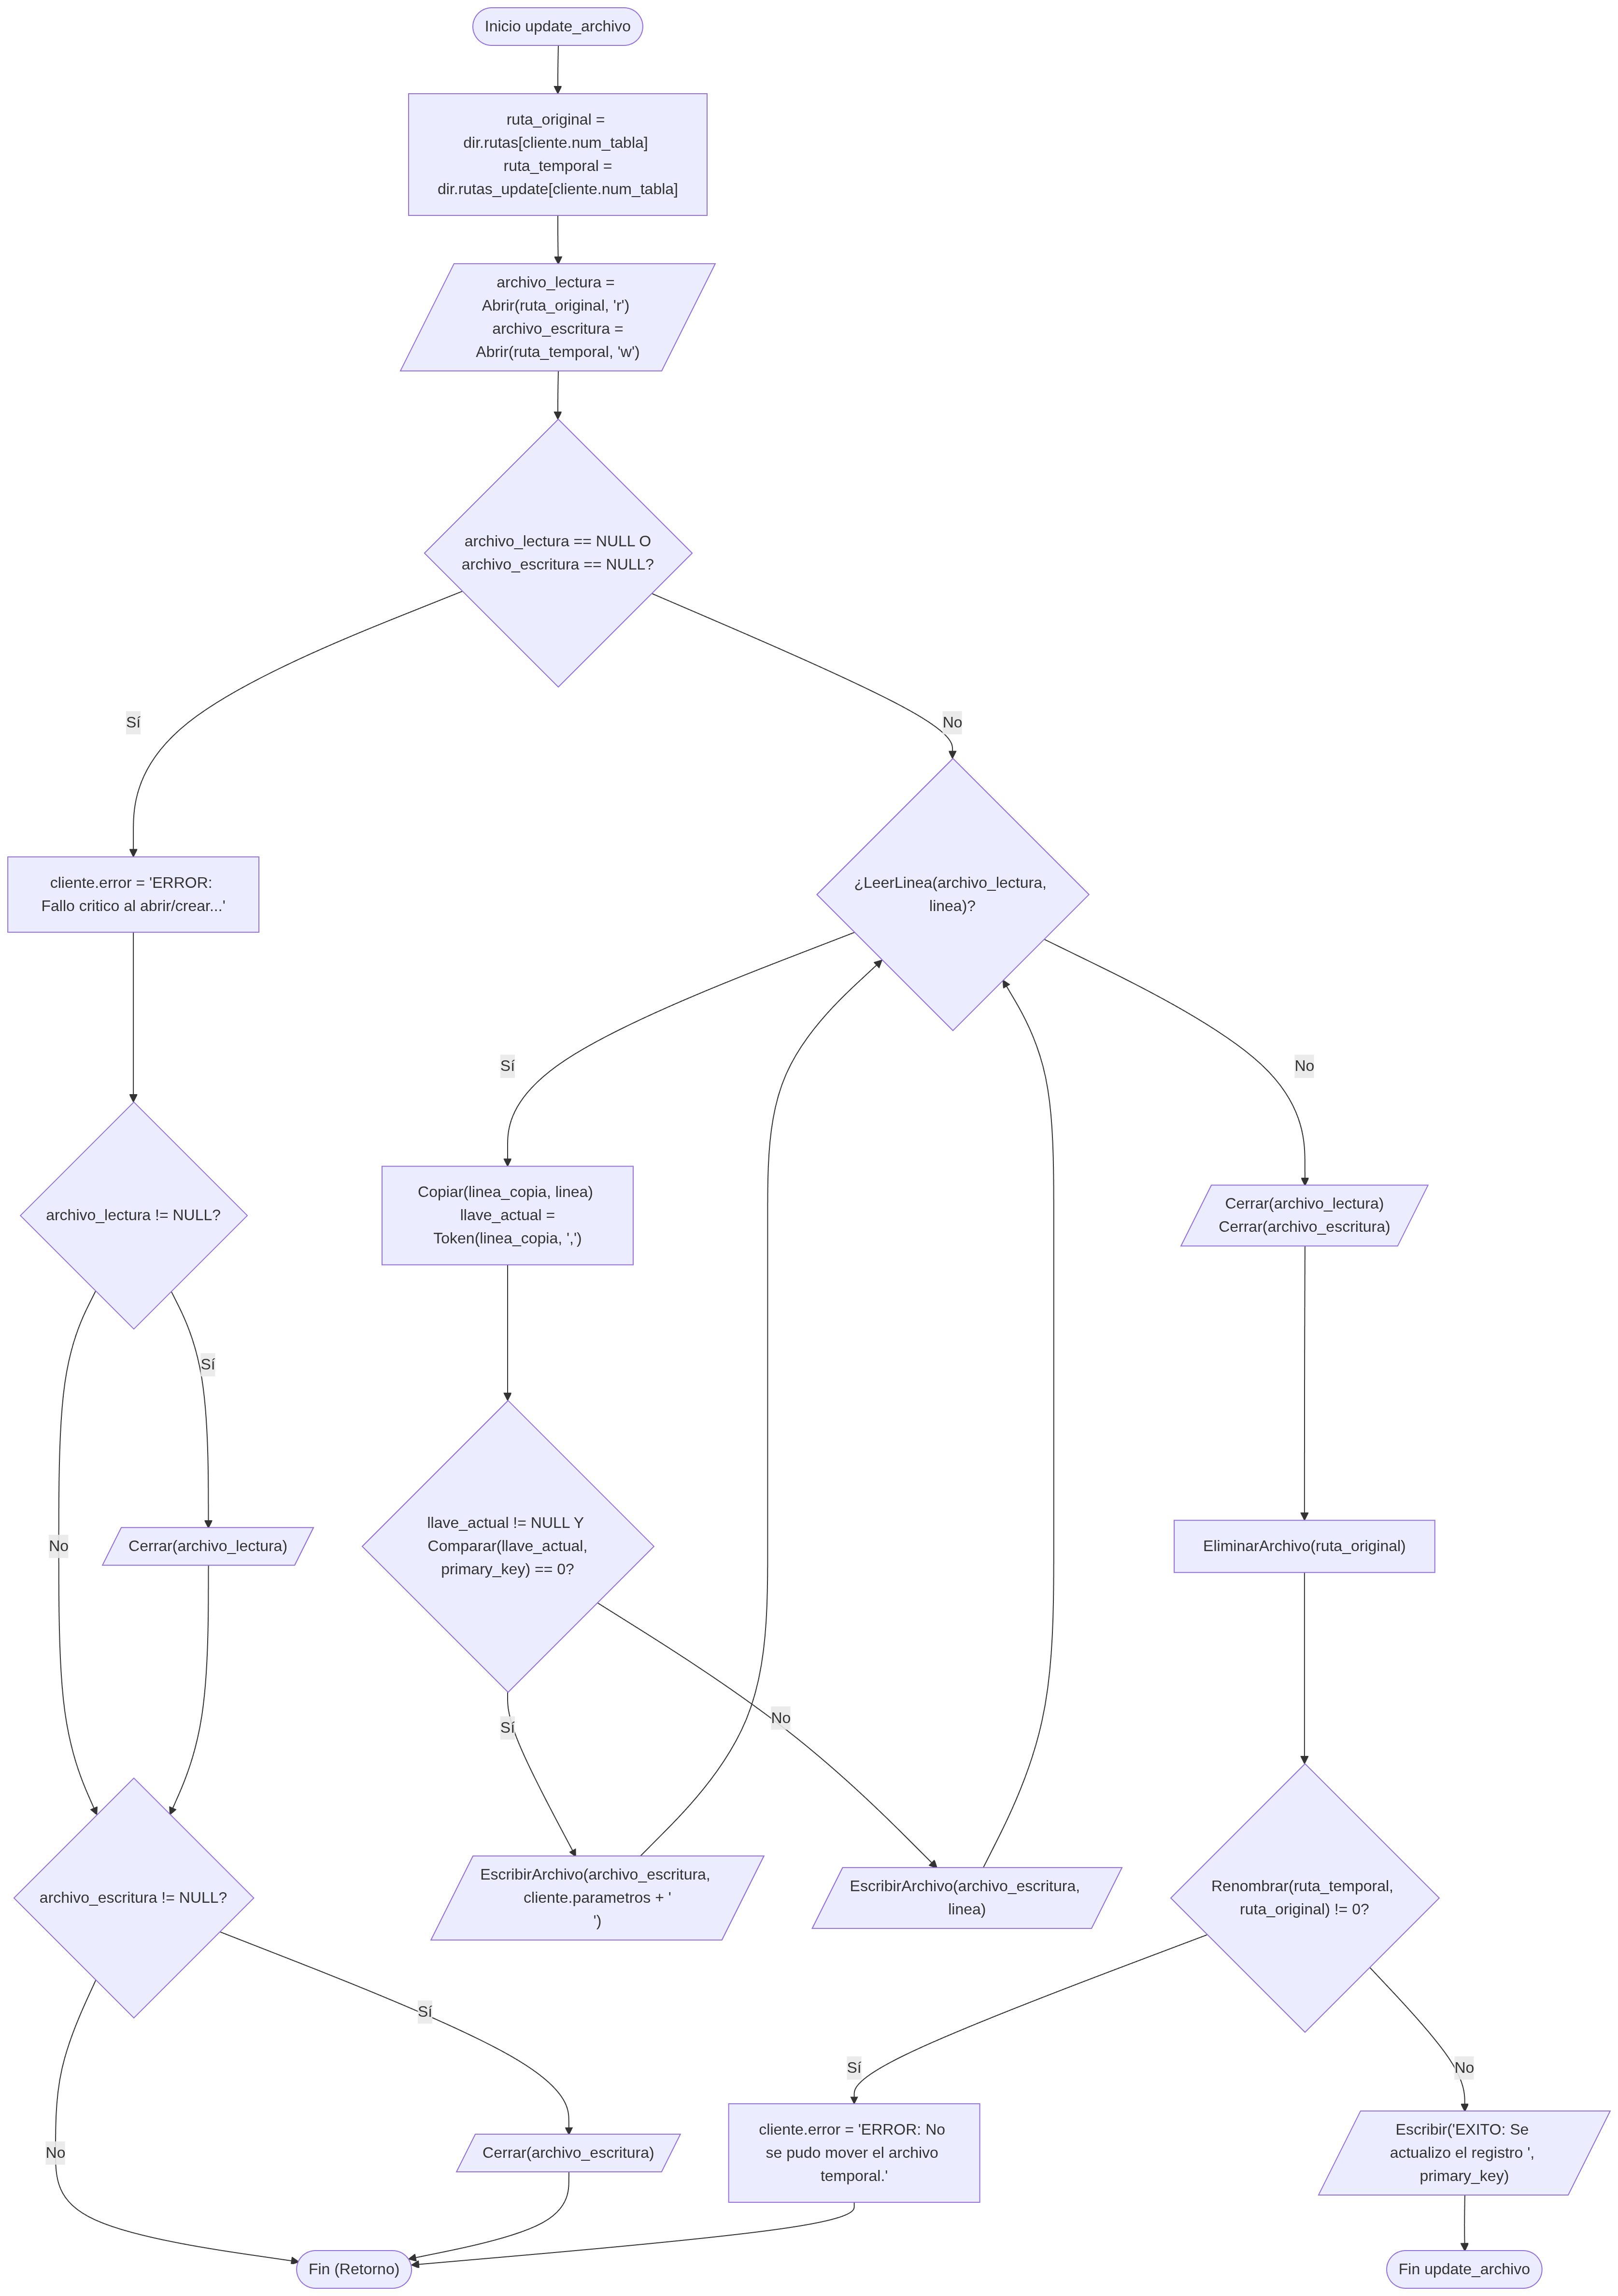
\includegraphics[width=0.8\textwidth]{update/update_archivo.png} 
    \caption{update.c/update\_archivo}
\end{figure}